% =====================================================================
% Caso de uso 1 (localização). Seção do capítulo de resultados, incluída
% em resultados.tex com % =====================================================================
% Caso de uso 1 (localização). Seção do capítulo de resultados, incluída
% em resultados.tex com % =====================================================================
% Caso de uso 1 (localização). Seção do capítulo de resultados, incluída
% em resultados.tex com % =====================================================================
% Caso de uso 1 (localização). Seção do capítulo de resultados, incluída
% em resultados.tex com \input{resultados_uc1}. Figuras em figuras/*.jpg.
% Incerteza: Moffat (1988) e Poiate Junior (apostila), chaves em referencias.bib.
% Trechos marcados com "CONFERIR" dependem de informação do autor.
% =====================================================================

\section{Caso de uso 1: localização}
\label{sec:res-localizacao}

O intervalo analisado vai de 29/09/2026 a 17/10/2026 e reúne 275 posições da \textit{tag}. As 32 primeiras, até 10/10, foram coletadas pela instância local do servidor, antes da implantação; as 243 seguintes, pela instância em produção. As duas instâncias usam o mesmo código de consulta e de filtragem. Entre 30/09 e 10/10 não há posições, porque o servidor local ficou desligado nesse período. % CONFERIR: motivo da lacuna
As posições estão em metros a partir do centro da cerca virtual, sem mapa de fundo, para não expor o endereço do local de teste.

A Figura~\ref{fig:uc1-trajeto} apresenta as posições em duas escalas. Em (a), o período de 10/10 a 17/10, com a \textit{tag} parada dentro da cerca de 310 m de raio. Em (b), o intervalo total, que inclui o deslocamento a pé feito pelo autor em 30/09.

\begin{figure}[htb]
  \centering
  \caption{Posições recebidas da \textit{tag} e cerca virtual: (a) período com a \textit{tag} parada; (b) intervalo total}
  \label{fig:uc1-trajeto}
  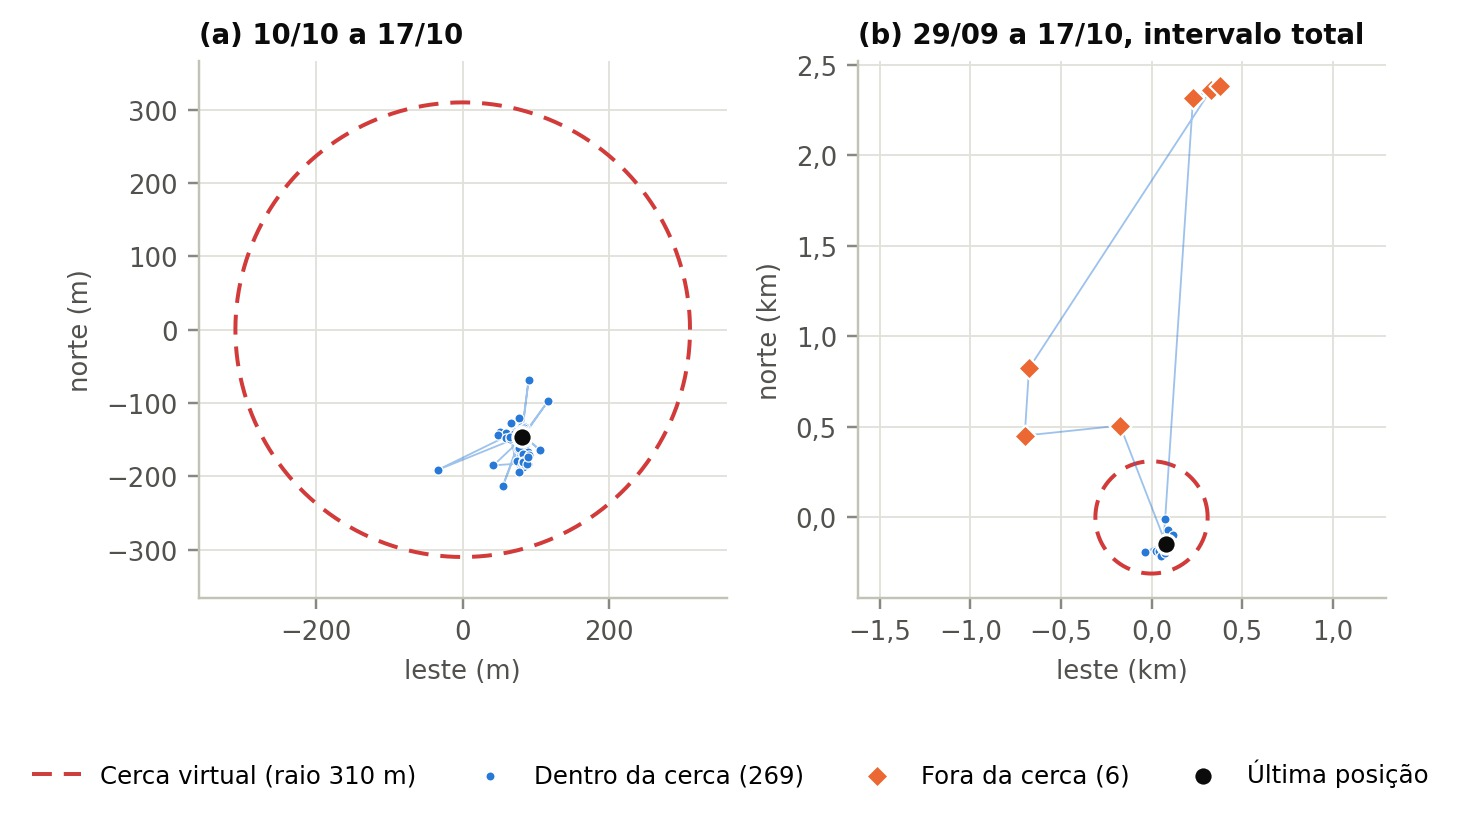
\includegraphics[width=\textwidth]{figuras/uc1_trajeto.jpg}
  \fonte{Elaborado pelo autor (2026).}
\end{figure}

Seis posições ficaram fora da cerca, todas em 30/09, entre 13h32 e 14h31, a até 2,41 km do centro. O site registrou o alerta de saída da cerca a partir da primeira delas: o cartão de localização do cavalo passou a indicar ``Fora da cerca'' e o alerta apareceu no sino do portal. Nas demais 269 posições a \textit{tag} estava dentro do raio.

A Figura~\ref{fig:uc1-dia} mostra quantas posições chegaram em cada dia. A quantidade variou de 6 a 75 por dia. A rede Find Hub depende de celulares Android que passem perto da \textit{tag}, e o servidor só registra o que a rede entrega.

\begin{figure}[htb]
  \centering
  \caption{Posições recebidas por dia, dentro e fora da cerca}
  \label{fig:uc1-dia}
  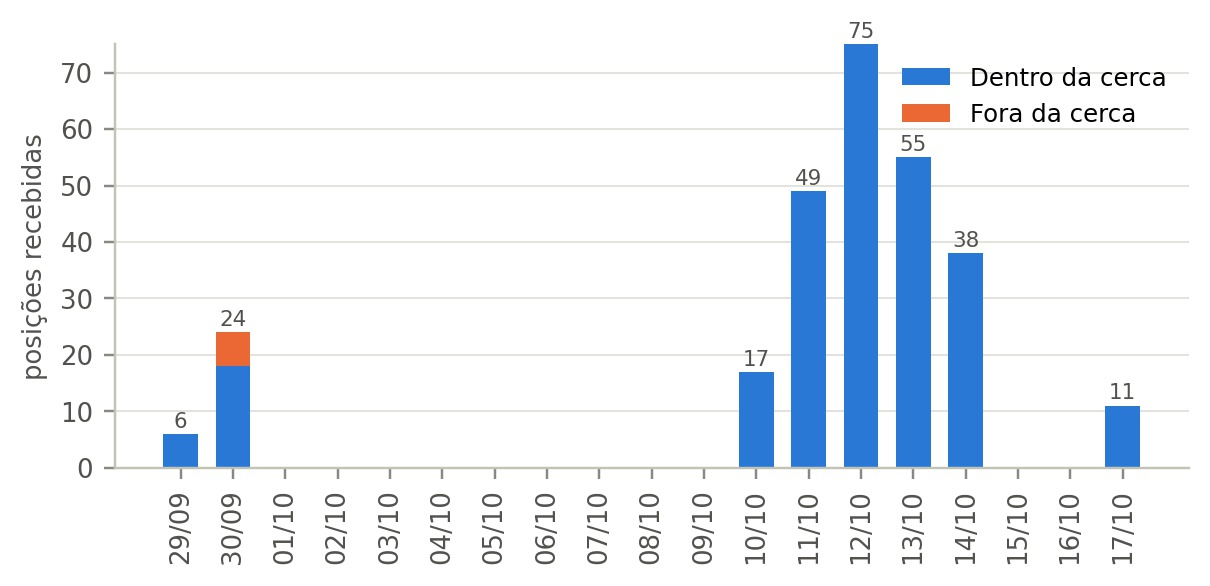
\includegraphics[width=\textwidth]{figuras/uc1_por_dia.jpg}
  \fonte{Elaborado pelo autor (2026).}
\end{figure}

A Figura~\ref{fig:uc1-intervalo} apresenta o intervalo entre posições consecutivas e a precisão informada pela rede em cada posição. O intervalo mediano foi de 16 min, e 90\% dos intervalos ficaram abaixo de 57 min; o maior intervalo, de 239 h, corresponde à lacuna entre 30/09 e 10/10. A precisão informada teve mediana de 75 m, e 46\% das posições chegaram com o valor máximo aceito pelo filtro do servidor, 100 m.

\begin{figure}[htb]
  \centering
  \caption{Intervalo entre posições consecutivas e precisão informada pela rede}
  \label{fig:uc1-intervalo}
  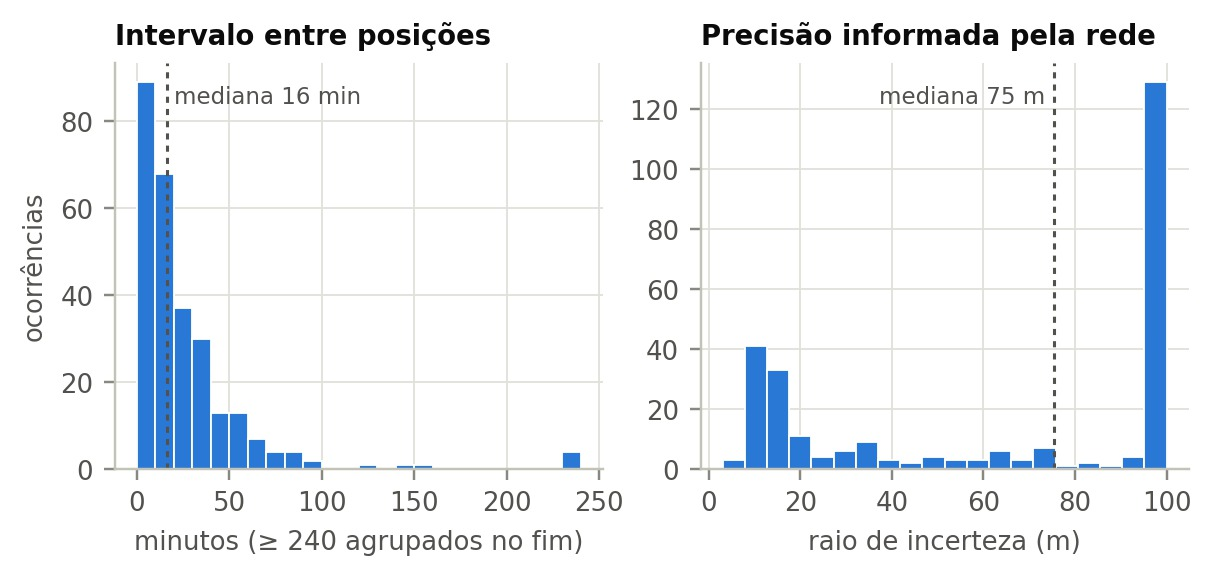
\includegraphics[width=\textwidth]{figuras/uc1_intervalo_precisao.jpg}
  \fonte{Elaborado pelo autor (2026).}
\end{figure}

\subsection{Incerteza da posição}
\label{sec:uc1-incerteza-posicao}

A incerteza foi avaliada pela análise de amostra única de \citeonline{moffat1988}: cada posição é uma leitura isolada, e a dispersão do sistema de medição é obtida de um experimento auxiliar feito em condição representativa. O experimento auxiliar foi o período de 10/10 a 17/10, com a \textit{tag} parada no mesmo ponto e 243 leituras. As coordenadas foram convertidas para metros nas direções leste ($x$) e norte ($y$), e o desvio-padrão amostral de cada direção foi $S_x = 9{,}6$~m e $S_y = 14{,}0$~m.

Com 242 graus de liberdade, a distribuição qui-quadrado limita o desvio-padrão da população a $0{,}92\,S \le \sigma \le 1{,}10\,S$, ao nível de 95\% \cite{moffat1988}. Foi adotado o valor mais provável, $\sigma = S$. A incerteza de uma leitura isolada, a 95\% de confiança (chance de 20 para 1), é
\begin{equation}
  \delta x = 2\sigma_x = 19{,}2~\text{m}, \qquad \delta y = 2\sigma_y = 27{,}9~\text{m}.
  \label{eq:uc1-incerteza-posicao}
\end{equation}
Com o limite superior de $\sigma$, os valores seriam 21,0 m e 30,6 m. Nos dados, 96,3\% das leituras ficaram dentro de $\pm\delta x$ e 92,2\% dentro de $\pm\delta y$. A distribuição não é gaussiana, pois 92\% das leituras na direção leste ficaram dentro de $\pm S_x$, e uma leitura isolada se afastou 121 m da média. A autocorrelação entre leituras consecutivas foi de $-0{,}001$ (leste) e $0{,}12$ (norte), e as leituras foram tratadas como independentes, condição exigida para a soma quadrática.

A Tabela~\ref{tab:uc1-ordens} separa a incerteza da posição nas três ordens de \citeonline{moffat1988}. A ordem zero corresponde à resolução dos valores recebidos, que chegam com $10^{-7}$ grau (cerca de 1,1 cm), e a incerteza instrumental é a metade da resolução \cite{poiate}. O horário de cada posição chega em segundos inteiros, com incerteza de 0,5 s. A primeira ordem é a dispersão medida no experimento auxiliar. Na ordem $N$ entraria o erro fixo da rede, isto é, a diferença entre a média das leituras e a posição verdadeira da \textit{tag}. Esse erro não foi medido, porque não havia uma referência de posição com incerteza menor; ele desloca todas as leituras da mesma forma, e por isso se cancela nas diferenças entre posições usadas na distância e na velocidade, mas afeta a verificação da cerca.

\begin{table}[htb]
  \centering
  \caption{Incerteza de uma posição a 95\% de confiança}
  \label{tab:uc1-ordens}
  \begin{tabular}{lrrl}
    \hline
    \textbf{Ordem} & \textbf{Leste (m)} & \textbf{Norte (m)} & \textbf{Origem} \\
    \hline
    Zero & 0,005 & 0,006 & resolução de $10^{-7}$ grau \\
    Primeira & 19,2 & 27,9 & experimento auxiliar, $2S$ \\
    $N$ & 19,2 & 27,9 & erro fixo da rede não avaliado \\
    \hline
  \end{tabular}
  \fonte{Elaborado pelo autor (2026).}
\end{table}

A ordem zero é cerca de 4 mil vezes menor que a primeira e foi desprezada, pois uma parcela menor que um terço da maior tem efeito pequeno na soma quadrática \cite{moffat1988}. Em 95,9\% das leituras paradas, a distância até a média ficou abaixo da precisão informada pela rede para aquela leitura, cuja mediana foi de 75 m. A precisão informada se comporta como um limite conservador, maior que a incerteza medida.

\subsection{Verificação da cerca com a incerteza}

A cerca virtual funciona como uma tolerância: a posição é aceita enquanto a distância $r$ até o centro não passa do raio $R = 310$~m. Seguindo \citeonline{poiate}, a incerteza de medição divide a faixa em três zonas. A zona de aceitação vai até $R - \delta r$, a zona de rejeição começa em $R + \delta r$ e, entre as duas, fica a zona de dúvida, onde a medição não permite afirmar se a \textit{tag} está dentro ou fora. A incerteza da distância ao centro vem da propagação das incertezas da Equação~\eqref{eq:uc1-incerteza-posicao}:
\begin{equation}
  \delta r = \sqrt{\left(\frac{x}{r}\,\delta x\right)^2 + \left(\frac{y}{r}\,\delta y\right)^2}.
  \label{eq:uc1-incerteza-raio}
\end{equation}

O maior valor de $\delta r$ entre as posições foi de 27,8 m, o que coloca a zona de dúvida entre 282 m e 338 m. A incerteza ficou abaixo de um décimo do intervalo de tolerância (31 m), critério de equilíbrio entre custo e qualidade recomendado por \citeonline{poiate}. A Figura~\ref{fig:uc1-zonas} mostra a distância de cada posição ao centro com as três zonas.

\begin{figure}[htb]
  \centering
  \caption{Distância das posições ao centro da cerca, com as zonas de aceitação, dúvida e rejeição}
  \label{fig:uc1-zonas}
  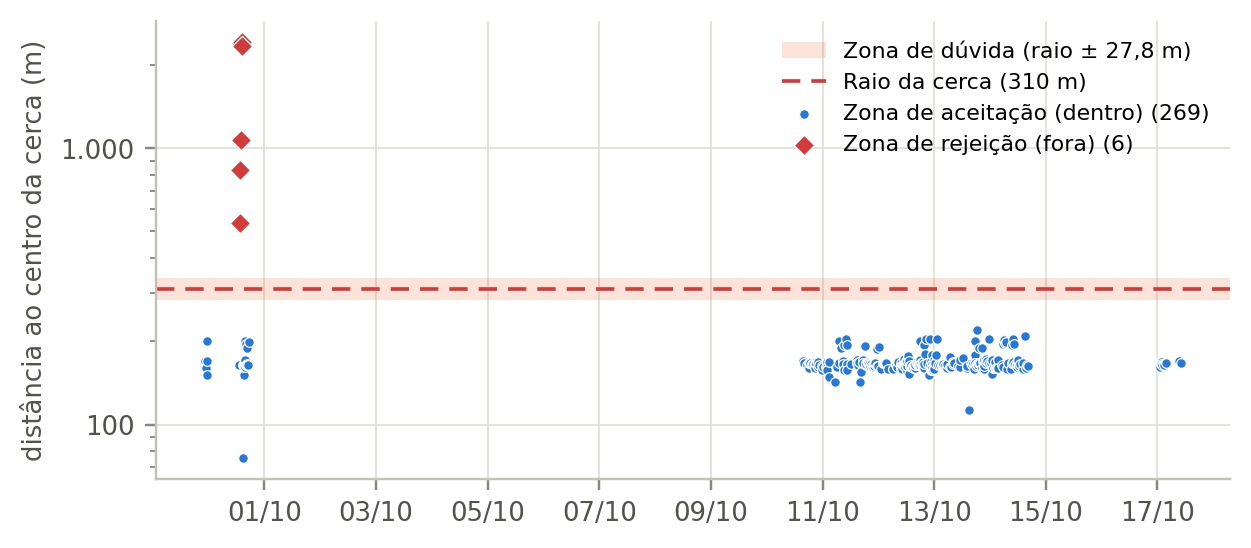
\includegraphics[width=\textwidth]{figuras/uc1_zonas.jpg}
  \fonte{Elaborado pelo autor (2026).}
\end{figure}

As 269 posições dentro da cerca ficaram a até 220 m do centro, na zona de aceitação. As seis posições de 30/09 ficaram a pelo menos 536 m, na zona de rejeição, e nenhuma posição caiu na zona de dúvida. O alerta de saída da cerca de 30/09 não depende, portanto, da incerteza da posição.

\subsection{Parâmetros calculados pelo site}

O site calcula, a partir das posições gravadas no banco, quatro parâmetros para o intervalo escolhido. A distância percorrida é a soma das distâncias entre posições consecutivas, $d = \sum_k s_k$. A velocidade média é essa distância dividida pelo tempo $T$ entre a primeira e a última posição. A velocidade máxima é a maior razão $s_k/\Delta t_k$ entre duas posições consecutivas. A aceleração média é a média das variações de velocidade entre trechos seguidos.

A incerteza desses resultados foi propagada pelo método da perturbação sequencial \cite{moffat1988}, aplicado à mesma função de cálculo do site. Cada entrada $X_i$ (latitude, longitude e horário de cada posição) foi aumentada e reduzida pela sua incerteza $\delta X_i$, uma de cada vez, e a contribuição $C_i$ foi tomada como a média de $|R_{i+} - R_0|$ e $|R_{i-} - R_0|$, porque o resultado não é linear nas posições. A incerteza do resultado é a soma quadrática das contribuições,
\begin{equation}
  \delta R = \sqrt{\sum_i C_i^2}, \qquad C_i \approx \frac{\partial R}{\partial X_i}\,\delta X_i,
  \label{eq:uc1-perturbacao}
\end{equation}
e tem o mesmo nível de confiança das entradas, 95\%. Para a velocidade média, a propagação analítica da apostila de \citeonline{poiate},
\begin{equation}
  \frac{\delta \bar v}{\bar v} = \sqrt{\left(\frac{\delta d}{d}\right)^2 + \left(\frac{\delta T}{T}\right)^2},
  \label{eq:uc1-vmed}
\end{equation}
com $\delta T = 1$~s (metade da resolução em cada extremo), deu o mesmo valor que a perturbação sequencial até a terceira casa. A parcela do horário foi desprezível em todos os resultados, exceto na velocidade máxima de 13/10, em que foi de 23 km/h contra 128 km/h da parcela das posições.

A soma de passos tem também um erro fixo, que \citeonline{moffat1988} classifica como erro conceitual: com a \textit{tag} parada, o ruído da posição gera passos de comprimento não nulo, e o site os soma como distância. Esse erro foi medido no experimento auxiliar, com 121 pares de leituras consecutivas sem leitura em comum. O passo médio foi de $(14{,}0 \pm 3{,}3)$~m, em que a incerteza é $t\,S/\sqrt{N}$, com $t = 1{,}98$ para 120 graus de liberdade. Para um intervalo com $k$ passos, o erro fixo é $B = k \times 14{,}0$~m, e a sua incerteza, $k \times 3{,}3$~m, somada de forma linear, porque o mesmo valor médio é usado em todos os passos. A distância corrigida é $d - B$, e a sua incerteza de ordem $N$ é a soma quadrática da incerteza propagada com a incerteza de $B$. Essa correção supõe a \textit{tag} parada em todos os passos e, nos dias com deslocamento, superestima o erro fixo. A velocidade média recebe a mesma correção, dividida por $T$.

A Figura~\ref{fig:uc1-parametros} apresenta, por dia, o valor calculado pelo site, a incerteza expandida e o erro fixo. Um valor foi considerado significativo quando superou a sua incerteza, isto é, quando a diferença em relação a zero (ou ao erro fixo, no caso da distância e da velocidade média) foi maior que a incerteza dessa diferença \cite{moffat1988}.

\begin{figure}[htb]
  \centering
  \caption{Parâmetros calculados pelo site por dia, com a incerteza expandida e o erro fixo}
  \label{fig:uc1-parametros}
  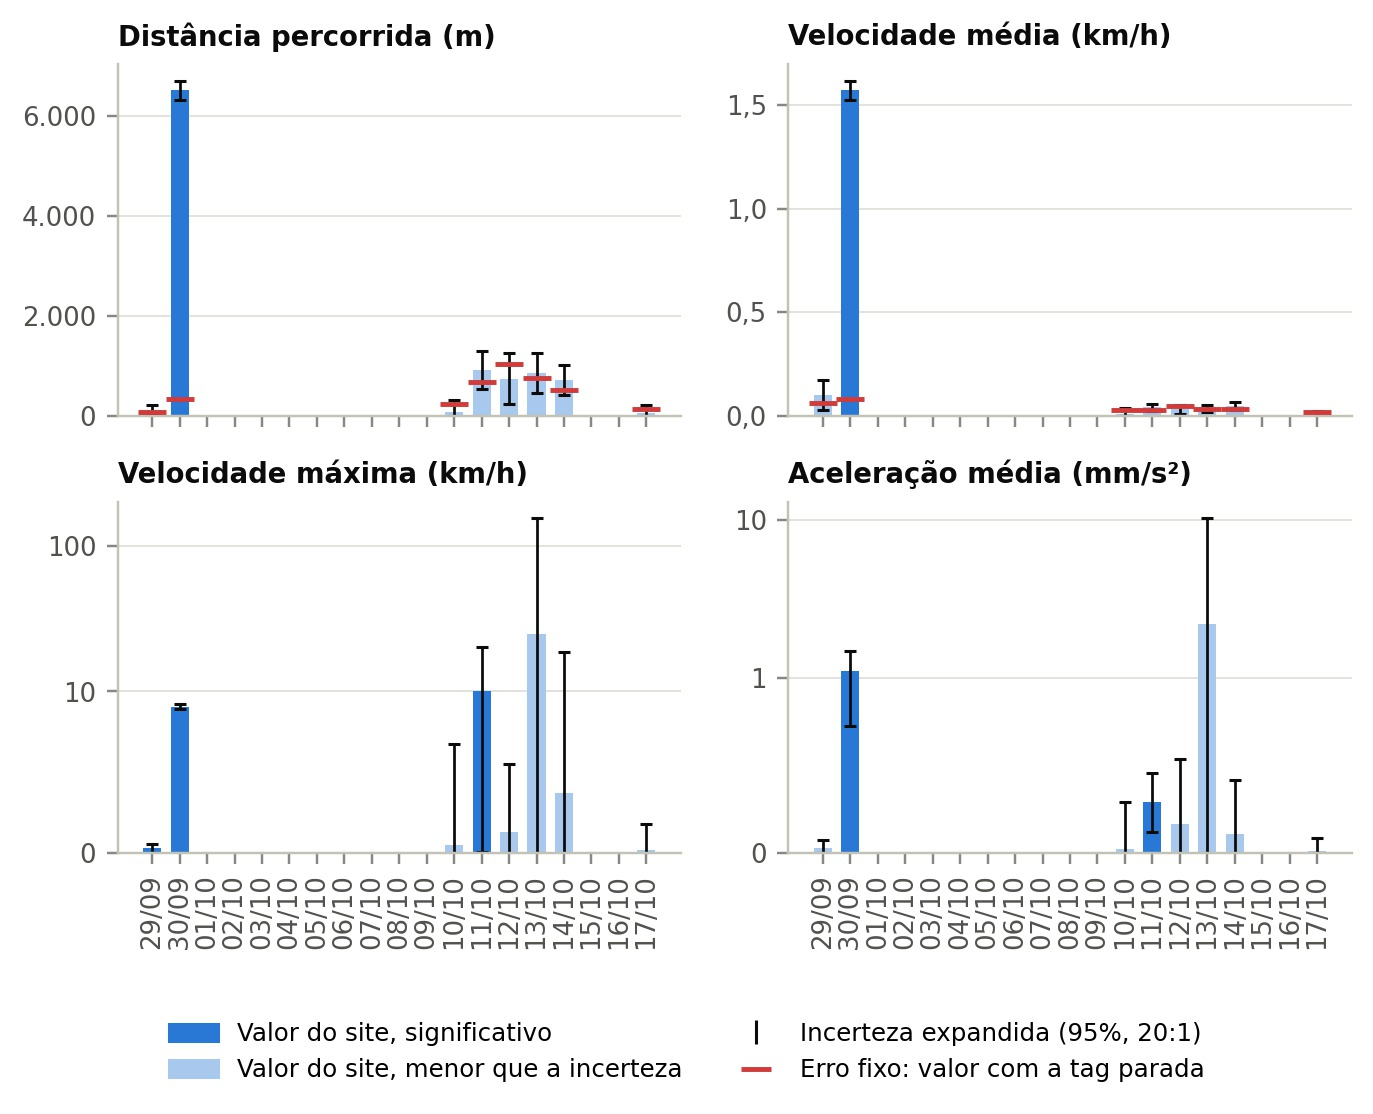
\includegraphics[width=\textwidth]{figuras/uc1_parametros.jpg}
  \fonte{Elaborado pelo autor (2026).}
\end{figure}

A Tabela~\ref{tab:uc1-dia30} reúne os resultados de 30/09, o dia com deslocamento, em 24 posições e 4 h 08 min. Todos os parâmetros foram significativos. A distância corrigida foi de $(6{,}19 \pm 0{,}19)$~km, com incerteza relativa de 3\%.

\begin{table}[htb]
  \centering
  \caption{Parâmetros de 30/09 a 95\% de confiança}
  \label{tab:uc1-dia30}
  \begin{tabular}{lrrr}
    \hline
    \textbf{Parâmetro} & \textbf{Valor do site} & \textbf{Erro fixo} & \textbf{Valor corrigido} \\
    \hline
    Distância percorrida & $(6{,}51 \pm 0{,}17)$ km & $(0{,}32 \pm 0{,}08)$ km & $(6{,}19 \pm 0{,}19)$ km \\
    Velocidade média & $(1{,}57 \pm 0{,}04)$ km/h & 0,08 km/h & $(1{,}50 \pm 0{,}05)$ km/h \\
    Velocidade máxima & $(9{,}0 \pm 0{,}2)$ km/h & --- & --- \\
    Aceleração média & $(1{,}1 \pm 0{,}4)$ mm/s² & --- & --- \\
    \hline
  \end{tabular}
  \fonte{Elaborado pelo autor (2026).}
\end{table}

Nos dias com a \textit{tag} parada, a distância corrigida foi compatível com zero. Em 11/10, por exemplo, o site somou 914 m, o erro fixo foi de 674 m e a distância corrigida, $(240 \pm 370)$~m. A velocidade máxima de 11/10, $(10 \pm 10)$~km/h, ficou no limite da significância, e a de 13/10, 24,7 km/h, teve incerteza de 130 km/h, porque vem de duas posições recebidas com poucos segundos de diferença. A Tabela~\ref{tab:uc1-total} reúne os parâmetros do intervalo total.

\begin{table}[htb]
  \centering
  \caption{Parâmetros calculados pelo site no intervalo total (29/09 a 17/10), a 95\% de confiança}
  \label{tab:uc1-total}
  \begin{tabular}{lrrr}
    \hline
    \textbf{Parâmetro} & \textbf{Valor do site} & \textbf{Erro fixo} & \textbf{Valor corrigido} \\
    \hline
    Distância percorrida & $(10{,}1 \pm 0{,}8)$ km & $(3{,}8 \pm 0{,}9)$ km & $(6{,}2 \pm 1{,}2)$ km \\
    Velocidade média & $(0{,}024 \pm 0{,}002)$ km/h & 0,009 km/h & $(0{,}015 \pm 0{,}003)$ km/h \\
    Velocidade máxima & $(25 \pm 130)$ km/h & --- & --- \\
    Aceleração média & $(0{,}7 \pm 1{,}7)$ mm/s² & --- & --- \\
    \hline
  \end{tabular}
  \fonte{Elaborado pelo autor (2026).}
\end{table}

A distância corrigida do intervalo total, $(6{,}2 \pm 1{,}2)$~km, coincide com a de 30/09: o restante dos 10,1 km somados pelo site corresponde ao ruído da posição nos dias parados. Um passo de comprimento próximo de zero tem incerteza de $\sqrt{2}\,\delta y = 39{,}5$~m, e 243 dos 274 passos do intervalo ficaram abaixo desse valor. A velocidade máxima e a aceleração média do intervalo total têm incerteza maior que o próprio valor e não permitem conclusões.

Com intervalos medianos de 16 min e incerteza de 19 m (leste) e 28 m (norte) a 95\% de confiança, a localização pela rede Find Hub atende à verificação da cerca virtual, sem posições na zona de dúvida. Para medir distância e velocidade em treinos, o cálculo do site precisaria descontar o erro fixo ou descartar passos menores que a incerteza de um passo, ou essas grandezas teriam de vir do acelerômetro.
. Figuras em figuras/*.jpg.
% Incerteza: Moffat (1988) e Poiate Junior (apostila), chaves em referencias.bib.
% Trechos marcados com "CONFERIR" dependem de informação do autor.
% =====================================================================

\section{Caso de uso 1: localização}
\label{sec:res-localizacao}

O intervalo analisado vai de 29/09/2026 a 17/10/2026 e reúne 275 posições da \textit{tag}. As 32 primeiras, até 10/10, foram coletadas pela instância local do servidor, antes da implantação; as 243 seguintes, pela instância em produção. As duas instâncias usam o mesmo código de consulta e de filtragem. Entre 30/09 e 10/10 não há posições, porque o servidor local ficou desligado nesse período. % CONFERIR: motivo da lacuna
As posições estão em metros a partir do centro da cerca virtual, sem mapa de fundo, para não expor o endereço do local de teste.

A Figura~\ref{fig:uc1-trajeto} apresenta as posições em duas escalas. Em (a), o período de 10/10 a 17/10, com a \textit{tag} parada dentro da cerca de 310 m de raio. Em (b), o intervalo total, que inclui o deslocamento a pé feito pelo autor em 30/09.

\begin{figure}[htb]
  \centering
  \caption{Posições recebidas da \textit{tag} e cerca virtual: (a) período com a \textit{tag} parada; (b) intervalo total}
  \label{fig:uc1-trajeto}
  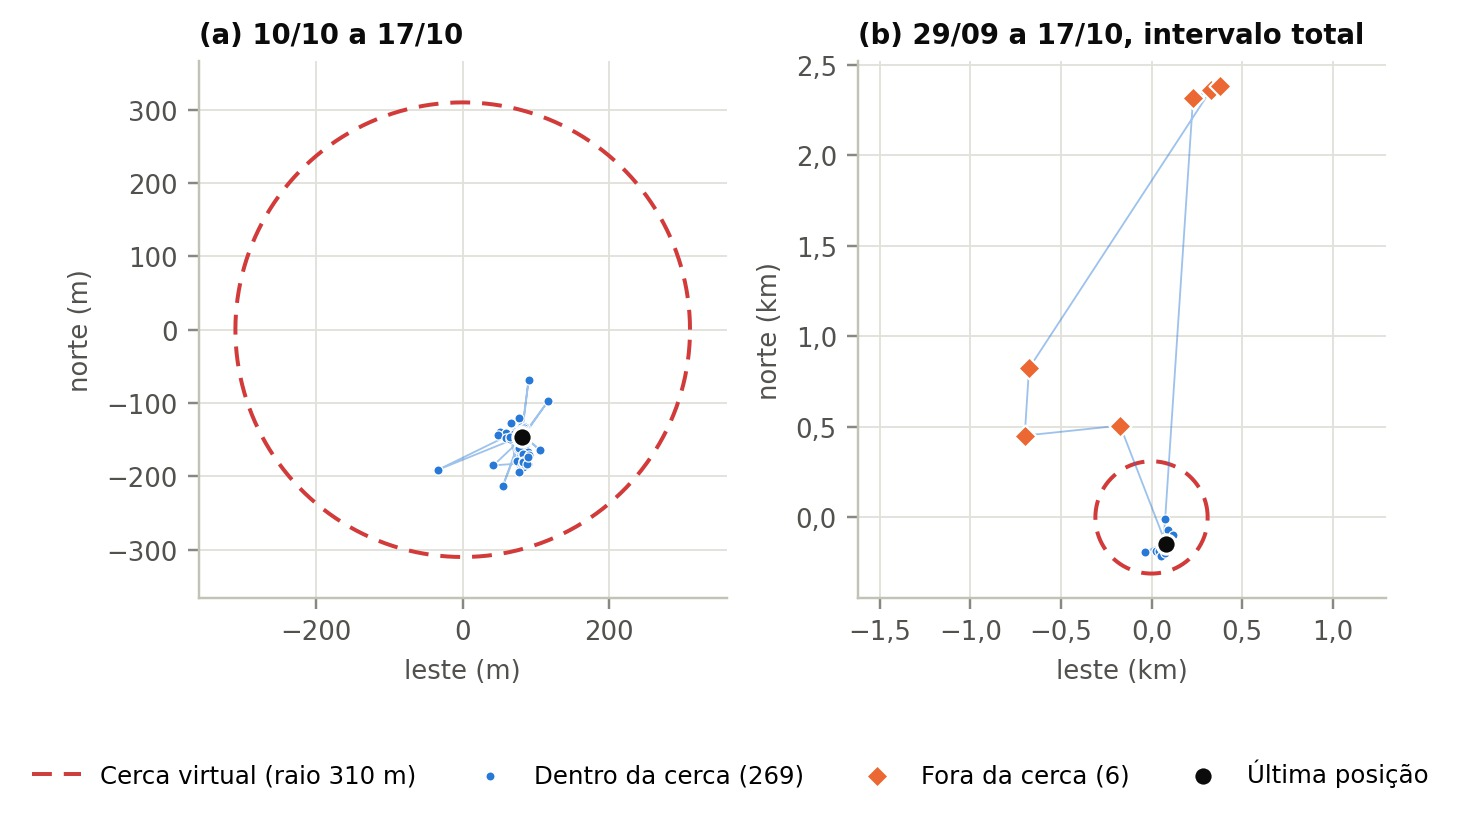
\includegraphics[width=\textwidth]{figuras/uc1_trajeto.jpg}
  \fonte{Elaborado pelo autor (2026).}
\end{figure}

Seis posições ficaram fora da cerca, todas em 30/09, entre 13h32 e 14h31, a até 2,41 km do centro. O site registrou o alerta de saída da cerca a partir da primeira delas: o cartão de localização do cavalo passou a indicar ``Fora da cerca'' e o alerta apareceu no sino do portal. Nas demais 269 posições a \textit{tag} estava dentro do raio.

A Figura~\ref{fig:uc1-dia} mostra quantas posições chegaram em cada dia. A quantidade variou de 6 a 75 por dia. A rede Find Hub depende de celulares Android que passem perto da \textit{tag}, e o servidor só registra o que a rede entrega.

\begin{figure}[htb]
  \centering
  \caption{Posições recebidas por dia, dentro e fora da cerca}
  \label{fig:uc1-dia}
  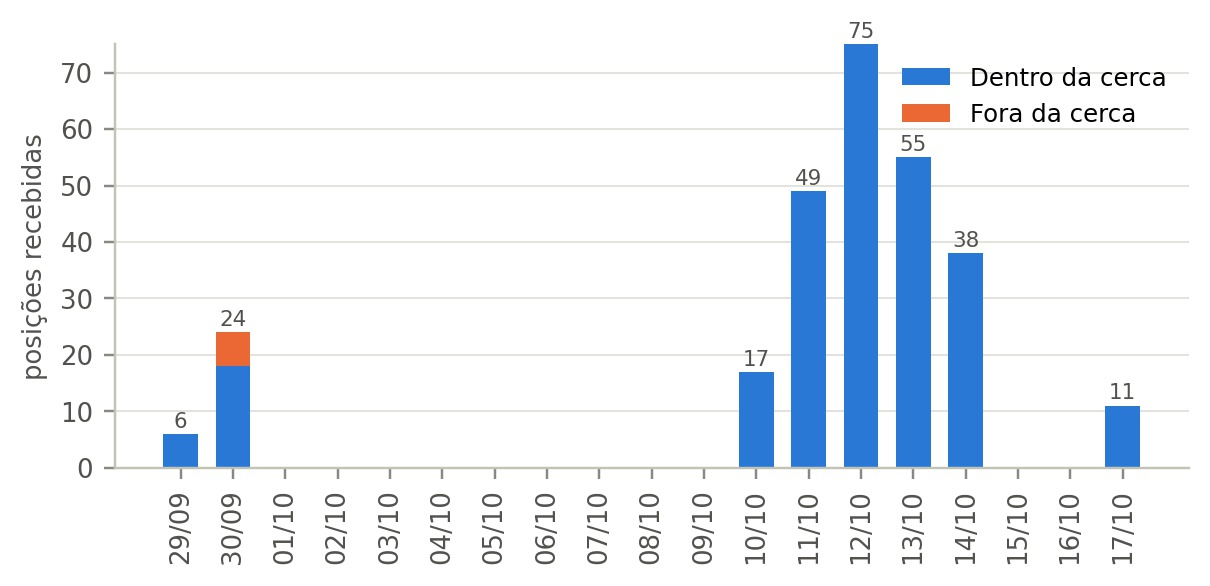
\includegraphics[width=\textwidth]{figuras/uc1_por_dia.jpg}
  \fonte{Elaborado pelo autor (2026).}
\end{figure}

A Figura~\ref{fig:uc1-intervalo} apresenta o intervalo entre posições consecutivas e a precisão informada pela rede em cada posição. O intervalo mediano foi de 16 min, e 90\% dos intervalos ficaram abaixo de 57 min; o maior intervalo, de 239 h, corresponde à lacuna entre 30/09 e 10/10. A precisão informada teve mediana de 75 m, e 46\% das posições chegaram com o valor máximo aceito pelo filtro do servidor, 100 m.

\begin{figure}[htb]
  \centering
  \caption{Intervalo entre posições consecutivas e precisão informada pela rede}
  \label{fig:uc1-intervalo}
  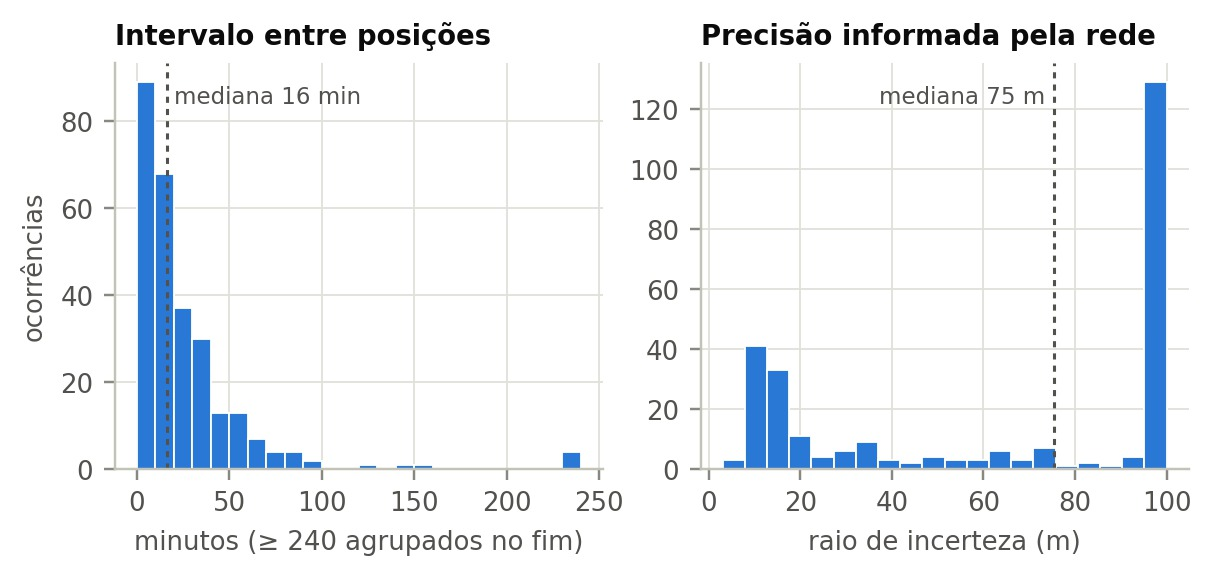
\includegraphics[width=\textwidth]{figuras/uc1_intervalo_precisao.jpg}
  \fonte{Elaborado pelo autor (2026).}
\end{figure}

\subsection{Incerteza da posição}
\label{sec:uc1-incerteza-posicao}

A incerteza foi avaliada pela análise de amostra única de \citeonline{moffat1988}: cada posição é uma leitura isolada, e a dispersão do sistema de medição é obtida de um experimento auxiliar feito em condição representativa. O experimento auxiliar foi o período de 10/10 a 17/10, com a \textit{tag} parada no mesmo ponto e 243 leituras. As coordenadas foram convertidas para metros nas direções leste ($x$) e norte ($y$), e o desvio-padrão amostral de cada direção foi $S_x = 9{,}6$~m e $S_y = 14{,}0$~m.

Com 242 graus de liberdade, a distribuição qui-quadrado limita o desvio-padrão da população a $0{,}92\,S \le \sigma \le 1{,}10\,S$, ao nível de 95\% \cite{moffat1988}. Foi adotado o valor mais provável, $\sigma = S$. A incerteza de uma leitura isolada, a 95\% de confiança (chance de 20 para 1), é
\begin{equation}
  \delta x = 2\sigma_x = 19{,}2~\text{m}, \qquad \delta y = 2\sigma_y = 27{,}9~\text{m}.
  \label{eq:uc1-incerteza-posicao}
\end{equation}
Com o limite superior de $\sigma$, os valores seriam 21,0 m e 30,6 m. Nos dados, 96,3\% das leituras ficaram dentro de $\pm\delta x$ e 92,2\% dentro de $\pm\delta y$. A distribuição não é gaussiana, pois 92\% das leituras na direção leste ficaram dentro de $\pm S_x$, e uma leitura isolada se afastou 121 m da média. A autocorrelação entre leituras consecutivas foi de $-0{,}001$ (leste) e $0{,}12$ (norte), e as leituras foram tratadas como independentes, condição exigida para a soma quadrática.

A Tabela~\ref{tab:uc1-ordens} separa a incerteza da posição nas três ordens de \citeonline{moffat1988}. A ordem zero corresponde à resolução dos valores recebidos, que chegam com $10^{-7}$ grau (cerca de 1,1 cm), e a incerteza instrumental é a metade da resolução \cite{poiate}. O horário de cada posição chega em segundos inteiros, com incerteza de 0,5 s. A primeira ordem é a dispersão medida no experimento auxiliar. Na ordem $N$ entraria o erro fixo da rede, isto é, a diferença entre a média das leituras e a posição verdadeira da \textit{tag}. Esse erro não foi medido, porque não havia uma referência de posição com incerteza menor; ele desloca todas as leituras da mesma forma, e por isso se cancela nas diferenças entre posições usadas na distância e na velocidade, mas afeta a verificação da cerca.

\begin{table}[htb]
  \centering
  \caption{Incerteza de uma posição a 95\% de confiança}
  \label{tab:uc1-ordens}
  \begin{tabular}{lrrl}
    \hline
    \textbf{Ordem} & \textbf{Leste (m)} & \textbf{Norte (m)} & \textbf{Origem} \\
    \hline
    Zero & 0,005 & 0,006 & resolução de $10^{-7}$ grau \\
    Primeira & 19,2 & 27,9 & experimento auxiliar, $2S$ \\
    $N$ & 19,2 & 27,9 & erro fixo da rede não avaliado \\
    \hline
  \end{tabular}
  \fonte{Elaborado pelo autor (2026).}
\end{table}

A ordem zero é cerca de 4 mil vezes menor que a primeira e foi desprezada, pois uma parcela menor que um terço da maior tem efeito pequeno na soma quadrática \cite{moffat1988}. Em 95,9\% das leituras paradas, a distância até a média ficou abaixo da precisão informada pela rede para aquela leitura, cuja mediana foi de 75 m. A precisão informada se comporta como um limite conservador, maior que a incerteza medida.

\subsection{Verificação da cerca com a incerteza}

A cerca virtual funciona como uma tolerância: a posição é aceita enquanto a distância $r$ até o centro não passa do raio $R = 310$~m. Seguindo \citeonline{poiate}, a incerteza de medição divide a faixa em três zonas. A zona de aceitação vai até $R - \delta r$, a zona de rejeição começa em $R + \delta r$ e, entre as duas, fica a zona de dúvida, onde a medição não permite afirmar se a \textit{tag} está dentro ou fora. A incerteza da distância ao centro vem da propagação das incertezas da Equação~\eqref{eq:uc1-incerteza-posicao}:
\begin{equation}
  \delta r = \sqrt{\left(\frac{x}{r}\,\delta x\right)^2 + \left(\frac{y}{r}\,\delta y\right)^2}.
  \label{eq:uc1-incerteza-raio}
\end{equation}

O maior valor de $\delta r$ entre as posições foi de 27,8 m, o que coloca a zona de dúvida entre 282 m e 338 m. A incerteza ficou abaixo de um décimo do intervalo de tolerância (31 m), critério de equilíbrio entre custo e qualidade recomendado por \citeonline{poiate}. A Figura~\ref{fig:uc1-zonas} mostra a distância de cada posição ao centro com as três zonas.

\begin{figure}[htb]
  \centering
  \caption{Distância das posições ao centro da cerca, com as zonas de aceitação, dúvida e rejeição}
  \label{fig:uc1-zonas}
  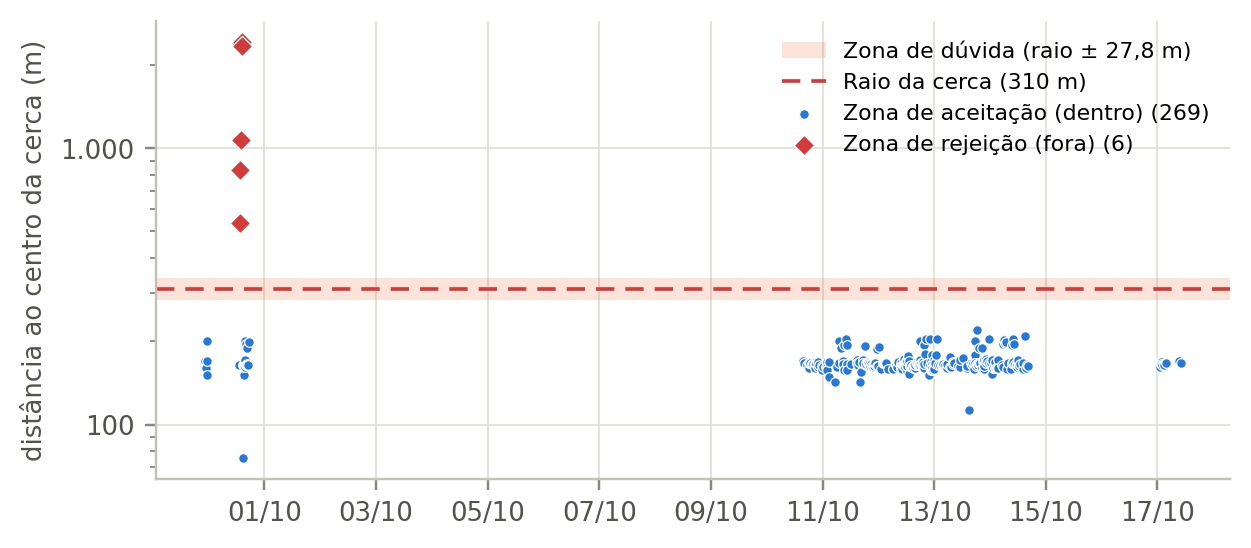
\includegraphics[width=\textwidth]{figuras/uc1_zonas.jpg}
  \fonte{Elaborado pelo autor (2026).}
\end{figure}

As 269 posições dentro da cerca ficaram a até 220 m do centro, na zona de aceitação. As seis posições de 30/09 ficaram a pelo menos 536 m, na zona de rejeição, e nenhuma posição caiu na zona de dúvida. O alerta de saída da cerca de 30/09 não depende, portanto, da incerteza da posição.

\subsection{Parâmetros calculados pelo site}

O site calcula, a partir das posições gravadas no banco, quatro parâmetros para o intervalo escolhido. A distância percorrida é a soma das distâncias entre posições consecutivas, $d = \sum_k s_k$. A velocidade média é essa distância dividida pelo tempo $T$ entre a primeira e a última posição. A velocidade máxima é a maior razão $s_k/\Delta t_k$ entre duas posições consecutivas. A aceleração média é a média das variações de velocidade entre trechos seguidos.

A incerteza desses resultados foi propagada pelo método da perturbação sequencial \cite{moffat1988}, aplicado à mesma função de cálculo do site. Cada entrada $X_i$ (latitude, longitude e horário de cada posição) foi aumentada e reduzida pela sua incerteza $\delta X_i$, uma de cada vez, e a contribuição $C_i$ foi tomada como a média de $|R_{i+} - R_0|$ e $|R_{i-} - R_0|$, porque o resultado não é linear nas posições. A incerteza do resultado é a soma quadrática das contribuições,
\begin{equation}
  \delta R = \sqrt{\sum_i C_i^2}, \qquad C_i \approx \frac{\partial R}{\partial X_i}\,\delta X_i,
  \label{eq:uc1-perturbacao}
\end{equation}
e tem o mesmo nível de confiança das entradas, 95\%. Para a velocidade média, a propagação analítica da apostila de \citeonline{poiate},
\begin{equation}
  \frac{\delta \bar v}{\bar v} = \sqrt{\left(\frac{\delta d}{d}\right)^2 + \left(\frac{\delta T}{T}\right)^2},
  \label{eq:uc1-vmed}
\end{equation}
com $\delta T = 1$~s (metade da resolução em cada extremo), deu o mesmo valor que a perturbação sequencial até a terceira casa. A parcela do horário foi desprezível em todos os resultados, exceto na velocidade máxima de 13/10, em que foi de 23 km/h contra 128 km/h da parcela das posições.

A soma de passos tem também um erro fixo, que \citeonline{moffat1988} classifica como erro conceitual: com a \textit{tag} parada, o ruído da posição gera passos de comprimento não nulo, e o site os soma como distância. Esse erro foi medido no experimento auxiliar, com 121 pares de leituras consecutivas sem leitura em comum. O passo médio foi de $(14{,}0 \pm 3{,}3)$~m, em que a incerteza é $t\,S/\sqrt{N}$, com $t = 1{,}98$ para 120 graus de liberdade. Para um intervalo com $k$ passos, o erro fixo é $B = k \times 14{,}0$~m, e a sua incerteza, $k \times 3{,}3$~m, somada de forma linear, porque o mesmo valor médio é usado em todos os passos. A distância corrigida é $d - B$, e a sua incerteza de ordem $N$ é a soma quadrática da incerteza propagada com a incerteza de $B$. Essa correção supõe a \textit{tag} parada em todos os passos e, nos dias com deslocamento, superestima o erro fixo. A velocidade média recebe a mesma correção, dividida por $T$.

A Figura~\ref{fig:uc1-parametros} apresenta, por dia, o valor calculado pelo site, a incerteza expandida e o erro fixo. Um valor foi considerado significativo quando superou a sua incerteza, isto é, quando a diferença em relação a zero (ou ao erro fixo, no caso da distância e da velocidade média) foi maior que a incerteza dessa diferença \cite{moffat1988}.

\begin{figure}[htb]
  \centering
  \caption{Parâmetros calculados pelo site por dia, com a incerteza expandida e o erro fixo}
  \label{fig:uc1-parametros}
  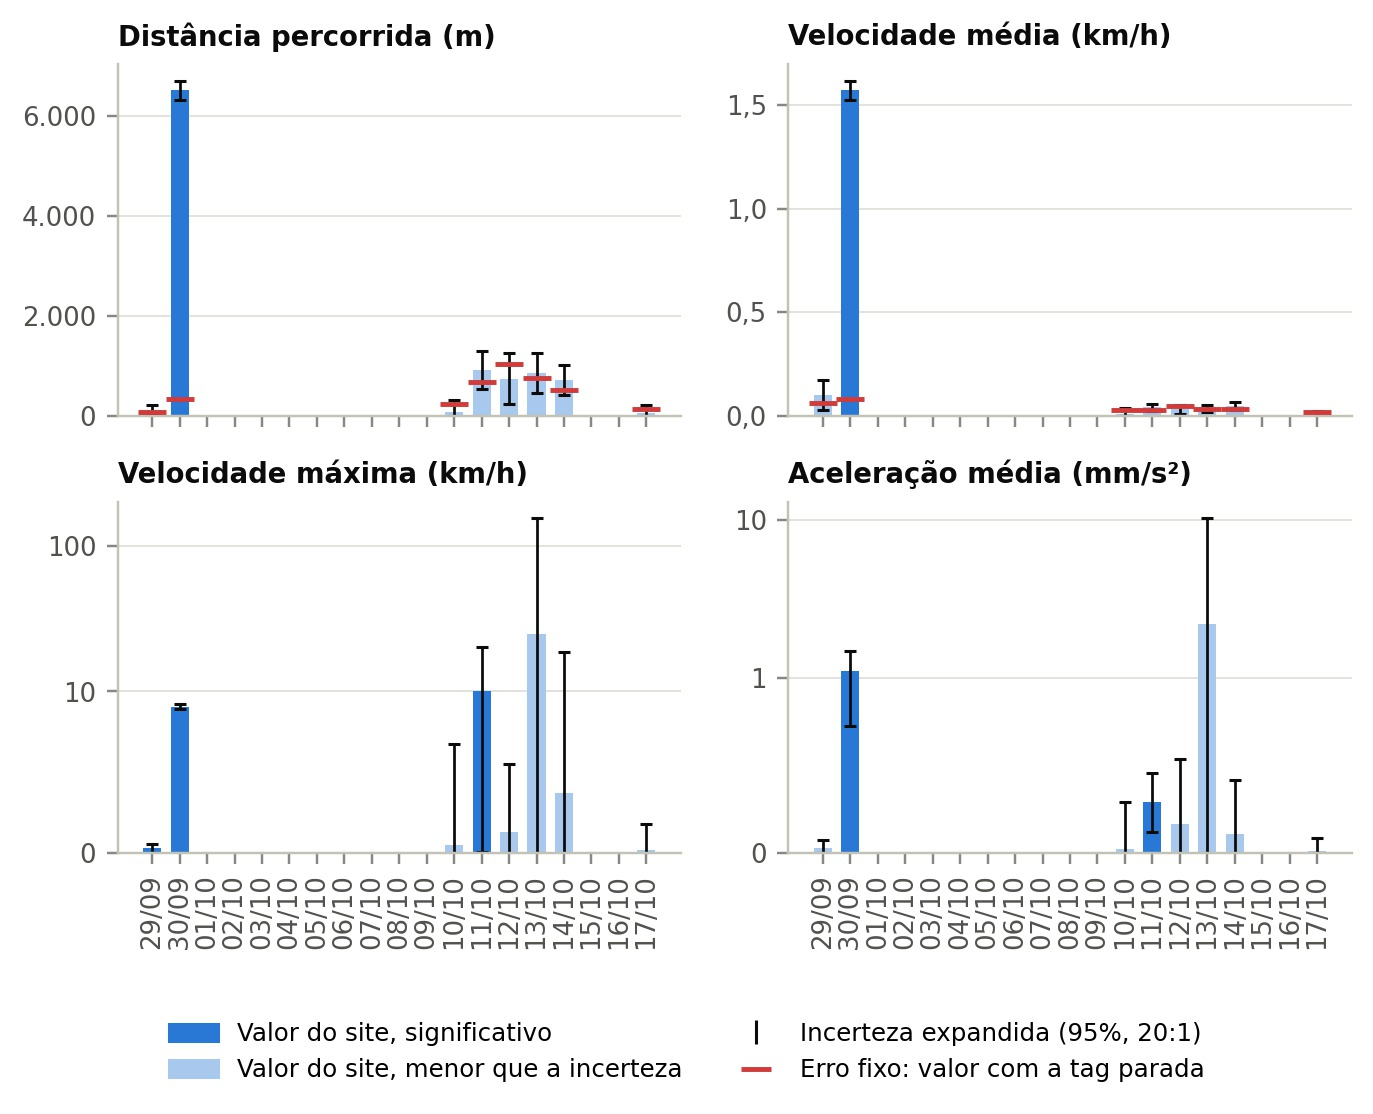
\includegraphics[width=\textwidth]{figuras/uc1_parametros.jpg}
  \fonte{Elaborado pelo autor (2026).}
\end{figure}

A Tabela~\ref{tab:uc1-dia30} reúne os resultados de 30/09, o dia com deslocamento, em 24 posições e 4 h 08 min. Todos os parâmetros foram significativos. A distância corrigida foi de $(6{,}19 \pm 0{,}19)$~km, com incerteza relativa de 3\%.

\begin{table}[htb]
  \centering
  \caption{Parâmetros de 30/09 a 95\% de confiança}
  \label{tab:uc1-dia30}
  \begin{tabular}{lrrr}
    \hline
    \textbf{Parâmetro} & \textbf{Valor do site} & \textbf{Erro fixo} & \textbf{Valor corrigido} \\
    \hline
    Distância percorrida & $(6{,}51 \pm 0{,}17)$ km & $(0{,}32 \pm 0{,}08)$ km & $(6{,}19 \pm 0{,}19)$ km \\
    Velocidade média & $(1{,}57 \pm 0{,}04)$ km/h & 0,08 km/h & $(1{,}50 \pm 0{,}05)$ km/h \\
    Velocidade máxima & $(9{,}0 \pm 0{,}2)$ km/h & --- & --- \\
    Aceleração média & $(1{,}1 \pm 0{,}4)$ mm/s² & --- & --- \\
    \hline
  \end{tabular}
  \fonte{Elaborado pelo autor (2026).}
\end{table}

Nos dias com a \textit{tag} parada, a distância corrigida foi compatível com zero. Em 11/10, por exemplo, o site somou 914 m, o erro fixo foi de 674 m e a distância corrigida, $(240 \pm 370)$~m. A velocidade máxima de 11/10, $(10 \pm 10)$~km/h, ficou no limite da significância, e a de 13/10, 24,7 km/h, teve incerteza de 130 km/h, porque vem de duas posições recebidas com poucos segundos de diferença. A Tabela~\ref{tab:uc1-total} reúne os parâmetros do intervalo total.

\begin{table}[htb]
  \centering
  \caption{Parâmetros calculados pelo site no intervalo total (29/09 a 17/10), a 95\% de confiança}
  \label{tab:uc1-total}
  \begin{tabular}{lrrr}
    \hline
    \textbf{Parâmetro} & \textbf{Valor do site} & \textbf{Erro fixo} & \textbf{Valor corrigido} \\
    \hline
    Distância percorrida & $(10{,}1 \pm 0{,}8)$ km & $(3{,}8 \pm 0{,}9)$ km & $(6{,}2 \pm 1{,}2)$ km \\
    Velocidade média & $(0{,}024 \pm 0{,}002)$ km/h & 0,009 km/h & $(0{,}015 \pm 0{,}003)$ km/h \\
    Velocidade máxima & $(25 \pm 130)$ km/h & --- & --- \\
    Aceleração média & $(0{,}7 \pm 1{,}7)$ mm/s² & --- & --- \\
    \hline
  \end{tabular}
  \fonte{Elaborado pelo autor (2026).}
\end{table}

A distância corrigida do intervalo total, $(6{,}2 \pm 1{,}2)$~km, coincide com a de 30/09: o restante dos 10,1 km somados pelo site corresponde ao ruído da posição nos dias parados. Um passo de comprimento próximo de zero tem incerteza de $\sqrt{2}\,\delta y = 39{,}5$~m, e 243 dos 274 passos do intervalo ficaram abaixo desse valor. A velocidade máxima e a aceleração média do intervalo total têm incerteza maior que o próprio valor e não permitem conclusões.

Com intervalos medianos de 16 min e incerteza de 19 m (leste) e 28 m (norte) a 95\% de confiança, a localização pela rede Find Hub atende à verificação da cerca virtual, sem posições na zona de dúvida. Para medir distância e velocidade em treinos, o cálculo do site precisaria descontar o erro fixo ou descartar passos menores que a incerteza de um passo, ou essas grandezas teriam de vir do acelerômetro.
. Figuras em figuras/*.jpg.
% Incerteza: Moffat (1988) e Poiate Junior (apostila), chaves em referencias.bib.
% Trechos marcados com "CONFERIR" dependem de informação do autor.
% =====================================================================

\section{Caso de uso 1: localização}
\label{sec:res-localizacao}

O intervalo analisado vai de 29/09/2026 a 17/10/2026 e reúne 275 posições da \textit{tag}. As 32 primeiras, até 10/10, foram coletadas pela instância local do servidor, antes da implantação; as 243 seguintes, pela instância em produção. As duas instâncias usam o mesmo código de consulta e de filtragem. Entre 30/09 e 10/10 não há posições, porque o servidor local ficou desligado nesse período. % CONFERIR: motivo da lacuna
As posições estão em metros a partir do centro da cerca virtual, sem mapa de fundo, para não expor o endereço do local de teste.

A Figura~\ref{fig:uc1-trajeto} apresenta as posições em duas escalas. Em (a), o período de 10/10 a 17/10, com a \textit{tag} parada dentro da cerca de 310 m de raio. Em (b), o intervalo total, que inclui o deslocamento a pé feito pelo autor em 30/09.

\begin{figure}[htb]
  \centering
  \caption{Posições recebidas da \textit{tag} e cerca virtual: (a) período com a \textit{tag} parada; (b) intervalo total}
  \label{fig:uc1-trajeto}
  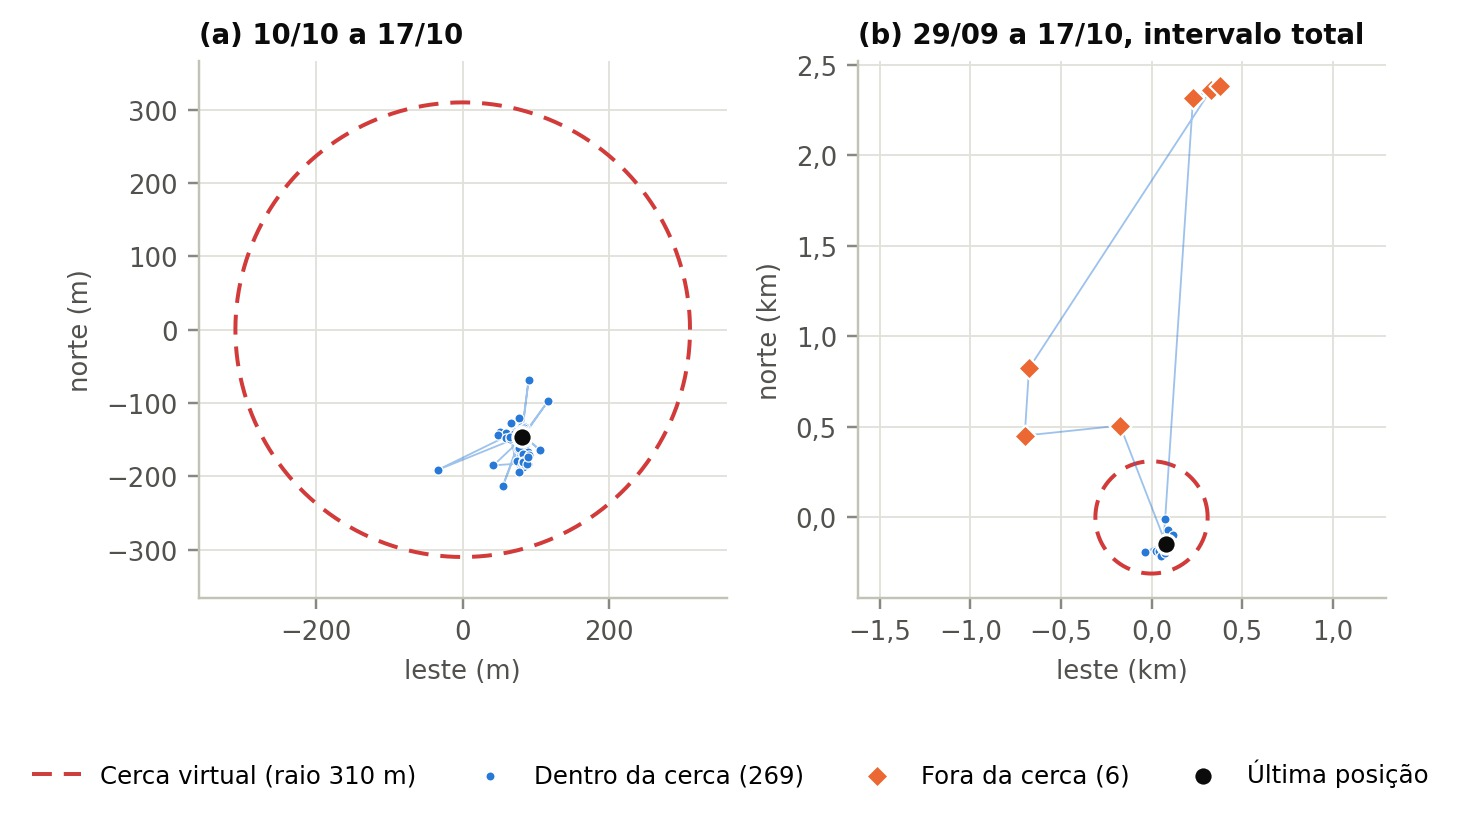
\includegraphics[width=\textwidth]{figuras/uc1_trajeto.jpg}
  \fonte{Elaborado pelo autor (2026).}
\end{figure}

Seis posições ficaram fora da cerca, todas em 30/09, entre 13h32 e 14h31, a até 2,41 km do centro. O site registrou o alerta de saída da cerca a partir da primeira delas: o cartão de localização do cavalo passou a indicar ``Fora da cerca'' e o alerta apareceu no sino do portal. Nas demais 269 posições a \textit{tag} estava dentro do raio.

A Figura~\ref{fig:uc1-dia} mostra quantas posições chegaram em cada dia. A quantidade variou de 6 a 75 por dia. A rede Find Hub depende de celulares Android que passem perto da \textit{tag}, e o servidor só registra o que a rede entrega.

\begin{figure}[htb]
  \centering
  \caption{Posições recebidas por dia, dentro e fora da cerca}
  \label{fig:uc1-dia}
  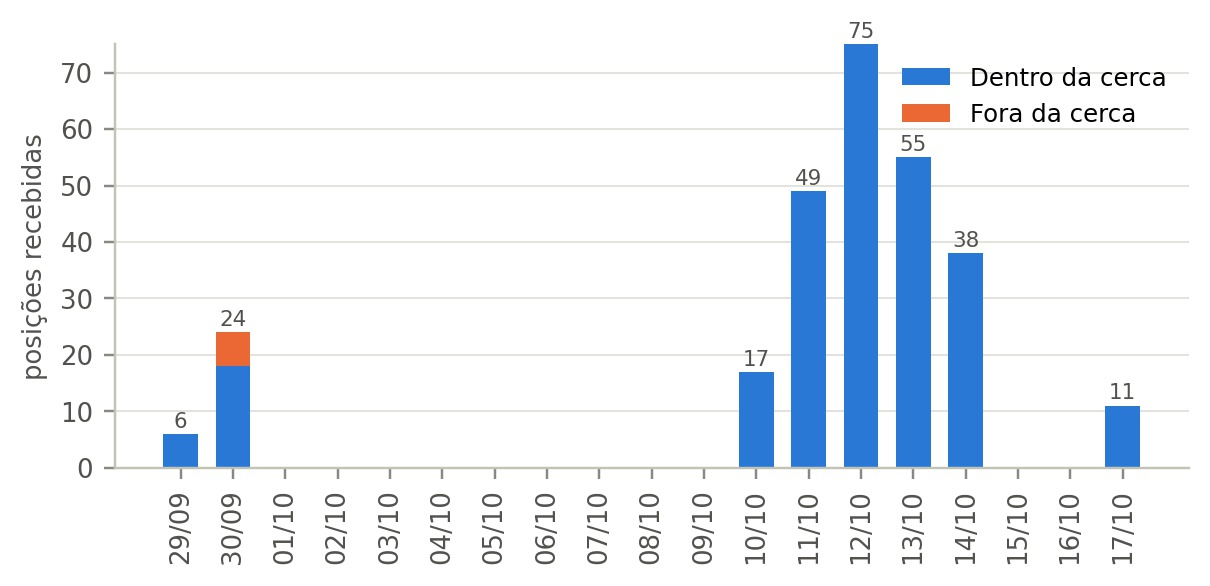
\includegraphics[width=\textwidth]{figuras/uc1_por_dia.jpg}
  \fonte{Elaborado pelo autor (2026).}
\end{figure}

A Figura~\ref{fig:uc1-intervalo} apresenta o intervalo entre posições consecutivas e a precisão informada pela rede em cada posição. O intervalo mediano foi de 16 min, e 90\% dos intervalos ficaram abaixo de 57 min; o maior intervalo, de 239 h, corresponde à lacuna entre 30/09 e 10/10. A precisão informada teve mediana de 75 m, e 46\% das posições chegaram com o valor máximo aceito pelo filtro do servidor, 100 m.

\begin{figure}[htb]
  \centering
  \caption{Intervalo entre posições consecutivas e precisão informada pela rede}
  \label{fig:uc1-intervalo}
  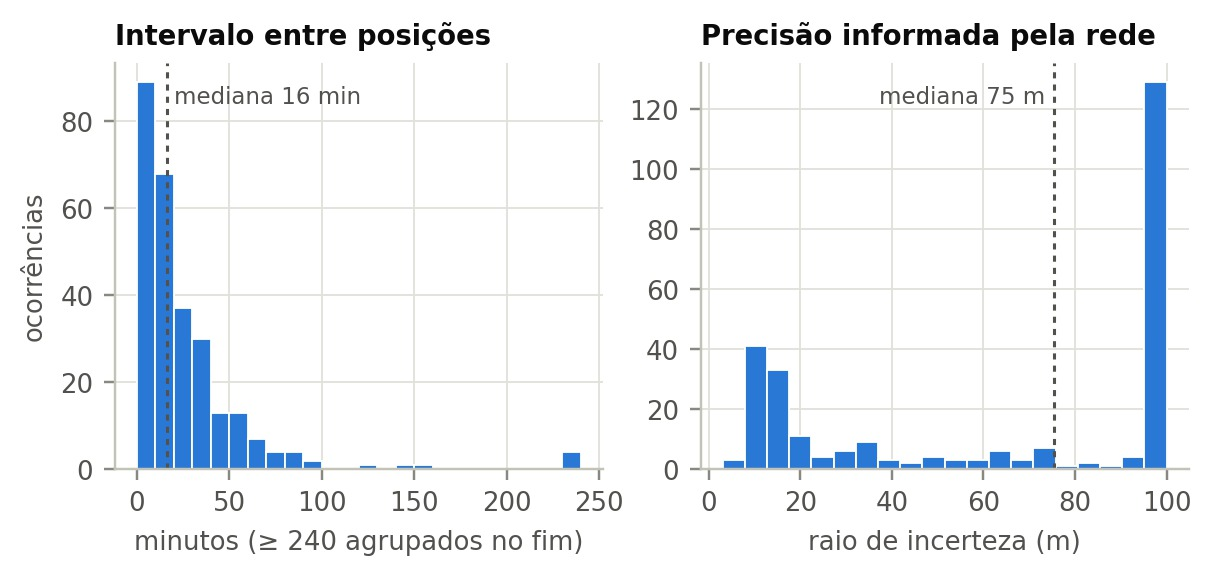
\includegraphics[width=\textwidth]{figuras/uc1_intervalo_precisao.jpg}
  \fonte{Elaborado pelo autor (2026).}
\end{figure}

\subsection{Incerteza da posição}
\label{sec:uc1-incerteza-posicao}

A incerteza foi avaliada pela análise de amostra única de \citeonline{moffat1988}: cada posição é uma leitura isolada, e a dispersão do sistema de medição é obtida de um experimento auxiliar feito em condição representativa. O experimento auxiliar foi o período de 10/10 a 17/10, com a \textit{tag} parada no mesmo ponto e 243 leituras. As coordenadas foram convertidas para metros nas direções leste ($x$) e norte ($y$), e o desvio-padrão amostral de cada direção foi $S_x = 9{,}6$~m e $S_y = 14{,}0$~m.

Com 242 graus de liberdade, a distribuição qui-quadrado limita o desvio-padrão da população a $0{,}92\,S \le \sigma \le 1{,}10\,S$, ao nível de 95\% \cite{moffat1988}. Foi adotado o valor mais provável, $\sigma = S$. A incerteza de uma leitura isolada, a 95\% de confiança (chance de 20 para 1), é
\begin{equation}
  \delta x = 2\sigma_x = 19{,}2~\text{m}, \qquad \delta y = 2\sigma_y = 27{,}9~\text{m}.
  \label{eq:uc1-incerteza-posicao}
\end{equation}
Com o limite superior de $\sigma$, os valores seriam 21,0 m e 30,6 m. Nos dados, 96,3\% das leituras ficaram dentro de $\pm\delta x$ e 92,2\% dentro de $\pm\delta y$. A distribuição não é gaussiana, pois 92\% das leituras na direção leste ficaram dentro de $\pm S_x$, e uma leitura isolada se afastou 121 m da média. A autocorrelação entre leituras consecutivas foi de $-0{,}001$ (leste) e $0{,}12$ (norte), e as leituras foram tratadas como independentes, condição exigida para a soma quadrática.

A Tabela~\ref{tab:uc1-ordens} separa a incerteza da posição nas três ordens de \citeonline{moffat1988}. A ordem zero corresponde à resolução dos valores recebidos, que chegam com $10^{-7}$ grau (cerca de 1,1 cm), e a incerteza instrumental é a metade da resolução \cite{poiate}. O horário de cada posição chega em segundos inteiros, com incerteza de 0,5 s. A primeira ordem é a dispersão medida no experimento auxiliar. Na ordem $N$ entraria o erro fixo da rede, isto é, a diferença entre a média das leituras e a posição verdadeira da \textit{tag}. Esse erro não foi medido, porque não havia uma referência de posição com incerteza menor; ele desloca todas as leituras da mesma forma, e por isso se cancela nas diferenças entre posições usadas na distância e na velocidade, mas afeta a verificação da cerca.

\begin{table}[htb]
  \centering
  \caption{Incerteza de uma posição a 95\% de confiança}
  \label{tab:uc1-ordens}
  \begin{tabular}{lrrl}
    \hline
    \textbf{Ordem} & \textbf{Leste (m)} & \textbf{Norte (m)} & \textbf{Origem} \\
    \hline
    Zero & 0,005 & 0,006 & resolução de $10^{-7}$ grau \\
    Primeira & 19,2 & 27,9 & experimento auxiliar, $2S$ \\
    $N$ & 19,2 & 27,9 & erro fixo da rede não avaliado \\
    \hline
  \end{tabular}
  \fonte{Elaborado pelo autor (2026).}
\end{table}

A ordem zero é cerca de 4 mil vezes menor que a primeira e foi desprezada, pois uma parcela menor que um terço da maior tem efeito pequeno na soma quadrática \cite{moffat1988}. Em 95,9\% das leituras paradas, a distância até a média ficou abaixo da precisão informada pela rede para aquela leitura, cuja mediana foi de 75 m. A precisão informada se comporta como um limite conservador, maior que a incerteza medida.

\subsection{Verificação da cerca com a incerteza}

A cerca virtual funciona como uma tolerância: a posição é aceita enquanto a distância $r$ até o centro não passa do raio $R = 310$~m. Seguindo \citeonline{poiate}, a incerteza de medição divide a faixa em três zonas. A zona de aceitação vai até $R - \delta r$, a zona de rejeição começa em $R + \delta r$ e, entre as duas, fica a zona de dúvida, onde a medição não permite afirmar se a \textit{tag} está dentro ou fora. A incerteza da distância ao centro vem da propagação das incertezas da Equação~\eqref{eq:uc1-incerteza-posicao}:
\begin{equation}
  \delta r = \sqrt{\left(\frac{x}{r}\,\delta x\right)^2 + \left(\frac{y}{r}\,\delta y\right)^2}.
  \label{eq:uc1-incerteza-raio}
\end{equation}

O maior valor de $\delta r$ entre as posições foi de 27,8 m, o que coloca a zona de dúvida entre 282 m e 338 m. A incerteza ficou abaixo de um décimo do intervalo de tolerância (31 m), critério de equilíbrio entre custo e qualidade recomendado por \citeonline{poiate}. A Figura~\ref{fig:uc1-zonas} mostra a distância de cada posição ao centro com as três zonas.

\begin{figure}[htb]
  \centering
  \caption{Distância das posições ao centro da cerca, com as zonas de aceitação, dúvida e rejeição}
  \label{fig:uc1-zonas}
  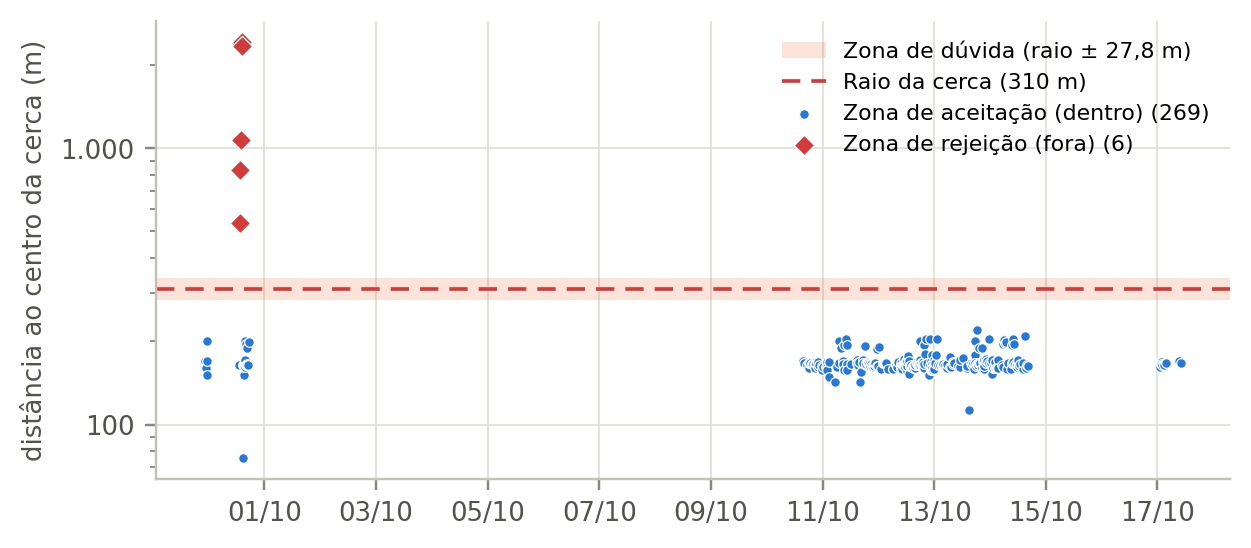
\includegraphics[width=\textwidth]{figuras/uc1_zonas.jpg}
  \fonte{Elaborado pelo autor (2026).}
\end{figure}

As 269 posições dentro da cerca ficaram a até 220 m do centro, na zona de aceitação. As seis posições de 30/09 ficaram a pelo menos 536 m, na zona de rejeição, e nenhuma posição caiu na zona de dúvida. O alerta de saída da cerca de 30/09 não depende, portanto, da incerteza da posição.

\subsection{Parâmetros calculados pelo site}

O site calcula, a partir das posições gravadas no banco, quatro parâmetros para o intervalo escolhido. A distância percorrida é a soma das distâncias entre posições consecutivas, $d = \sum_k s_k$. A velocidade média é essa distância dividida pelo tempo $T$ entre a primeira e a última posição. A velocidade máxima é a maior razão $s_k/\Delta t_k$ entre duas posições consecutivas. A aceleração média é a média das variações de velocidade entre trechos seguidos.

A incerteza desses resultados foi propagada pelo método da perturbação sequencial \cite{moffat1988}, aplicado à mesma função de cálculo do site. Cada entrada $X_i$ (latitude, longitude e horário de cada posição) foi aumentada e reduzida pela sua incerteza $\delta X_i$, uma de cada vez, e a contribuição $C_i$ foi tomada como a média de $|R_{i+} - R_0|$ e $|R_{i-} - R_0|$, porque o resultado não é linear nas posições. A incerteza do resultado é a soma quadrática das contribuições,
\begin{equation}
  \delta R = \sqrt{\sum_i C_i^2}, \qquad C_i \approx \frac{\partial R}{\partial X_i}\,\delta X_i,
  \label{eq:uc1-perturbacao}
\end{equation}
e tem o mesmo nível de confiança das entradas, 95\%. Para a velocidade média, a propagação analítica da apostila de \citeonline{poiate},
\begin{equation}
  \frac{\delta \bar v}{\bar v} = \sqrt{\left(\frac{\delta d}{d}\right)^2 + \left(\frac{\delta T}{T}\right)^2},
  \label{eq:uc1-vmed}
\end{equation}
com $\delta T = 1$~s (metade da resolução em cada extremo), deu o mesmo valor que a perturbação sequencial até a terceira casa. A parcela do horário foi desprezível em todos os resultados, exceto na velocidade máxima de 13/10, em que foi de 23 km/h contra 128 km/h da parcela das posições.

A soma de passos tem também um erro fixo, que \citeonline{moffat1988} classifica como erro conceitual: com a \textit{tag} parada, o ruído da posição gera passos de comprimento não nulo, e o site os soma como distância. Esse erro foi medido no experimento auxiliar, com 121 pares de leituras consecutivas sem leitura em comum. O passo médio foi de $(14{,}0 \pm 3{,}3)$~m, em que a incerteza é $t\,S/\sqrt{N}$, com $t = 1{,}98$ para 120 graus de liberdade. Para um intervalo com $k$ passos, o erro fixo é $B = k \times 14{,}0$~m, e a sua incerteza, $k \times 3{,}3$~m, somada de forma linear, porque o mesmo valor médio é usado em todos os passos. A distância corrigida é $d - B$, e a sua incerteza de ordem $N$ é a soma quadrática da incerteza propagada com a incerteza de $B$. Essa correção supõe a \textit{tag} parada em todos os passos e, nos dias com deslocamento, superestima o erro fixo. A velocidade média recebe a mesma correção, dividida por $T$.

A Figura~\ref{fig:uc1-parametros} apresenta, por dia, o valor calculado pelo site, a incerteza expandida e o erro fixo. Um valor foi considerado significativo quando superou a sua incerteza, isto é, quando a diferença em relação a zero (ou ao erro fixo, no caso da distância e da velocidade média) foi maior que a incerteza dessa diferença \cite{moffat1988}.

\begin{figure}[htb]
  \centering
  \caption{Parâmetros calculados pelo site por dia, com a incerteza expandida e o erro fixo}
  \label{fig:uc1-parametros}
  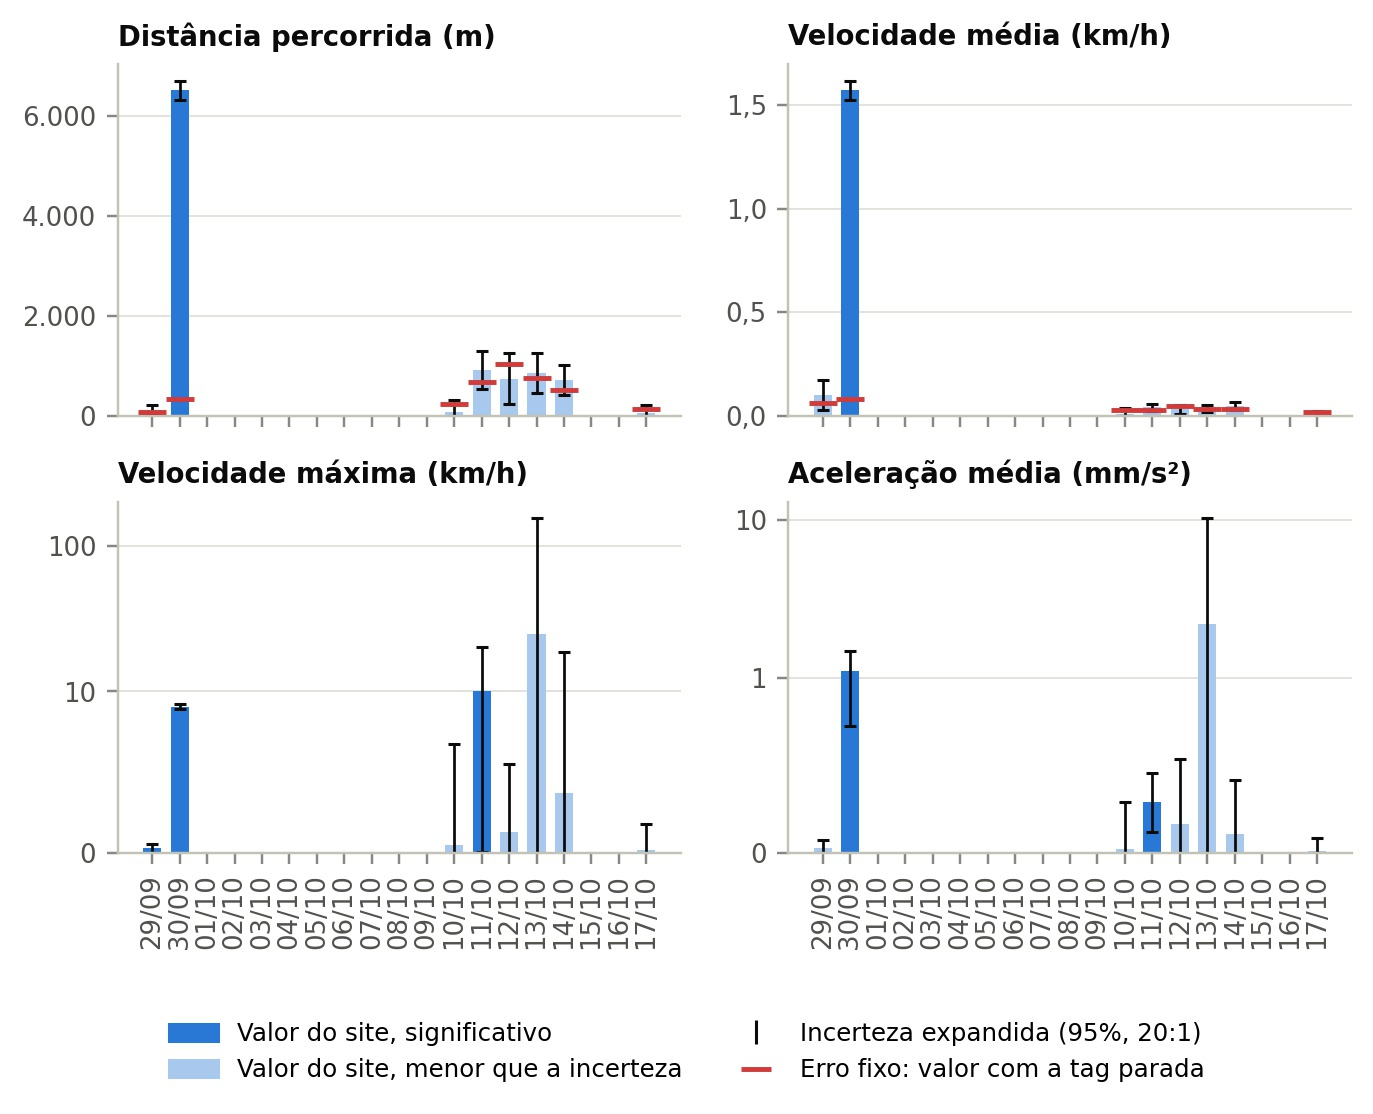
\includegraphics[width=\textwidth]{figuras/uc1_parametros.jpg}
  \fonte{Elaborado pelo autor (2026).}
\end{figure}

A Tabela~\ref{tab:uc1-dia30} reúne os resultados de 30/09, o dia com deslocamento, em 24 posições e 4 h 08 min. Todos os parâmetros foram significativos. A distância corrigida foi de $(6{,}19 \pm 0{,}19)$~km, com incerteza relativa de 3\%.

\begin{table}[htb]
  \centering
  \caption{Parâmetros de 30/09 a 95\% de confiança}
  \label{tab:uc1-dia30}
  \begin{tabular}{lrrr}
    \hline
    \textbf{Parâmetro} & \textbf{Valor do site} & \textbf{Erro fixo} & \textbf{Valor corrigido} \\
    \hline
    Distância percorrida & $(6{,}51 \pm 0{,}17)$ km & $(0{,}32 \pm 0{,}08)$ km & $(6{,}19 \pm 0{,}19)$ km \\
    Velocidade média & $(1{,}57 \pm 0{,}04)$ km/h & 0,08 km/h & $(1{,}50 \pm 0{,}05)$ km/h \\
    Velocidade máxima & $(9{,}0 \pm 0{,}2)$ km/h & --- & --- \\
    Aceleração média & $(1{,}1 \pm 0{,}4)$ mm/s² & --- & --- \\
    \hline
  \end{tabular}
  \fonte{Elaborado pelo autor (2026).}
\end{table}

Nos dias com a \textit{tag} parada, a distância corrigida foi compatível com zero. Em 11/10, por exemplo, o site somou 914 m, o erro fixo foi de 674 m e a distância corrigida, $(240 \pm 370)$~m. A velocidade máxima de 11/10, $(10 \pm 10)$~km/h, ficou no limite da significância, e a de 13/10, 24,7 km/h, teve incerteza de 130 km/h, porque vem de duas posições recebidas com poucos segundos de diferença. A Tabela~\ref{tab:uc1-total} reúne os parâmetros do intervalo total.

\begin{table}[htb]
  \centering
  \caption{Parâmetros calculados pelo site no intervalo total (29/09 a 17/10), a 95\% de confiança}
  \label{tab:uc1-total}
  \begin{tabular}{lrrr}
    \hline
    \textbf{Parâmetro} & \textbf{Valor do site} & \textbf{Erro fixo} & \textbf{Valor corrigido} \\
    \hline
    Distância percorrida & $(10{,}1 \pm 0{,}8)$ km & $(3{,}8 \pm 0{,}9)$ km & $(6{,}2 \pm 1{,}2)$ km \\
    Velocidade média & $(0{,}024 \pm 0{,}002)$ km/h & 0,009 km/h & $(0{,}015 \pm 0{,}003)$ km/h \\
    Velocidade máxima & $(25 \pm 130)$ km/h & --- & --- \\
    Aceleração média & $(0{,}7 \pm 1{,}7)$ mm/s² & --- & --- \\
    \hline
  \end{tabular}
  \fonte{Elaborado pelo autor (2026).}
\end{table}

A distância corrigida do intervalo total, $(6{,}2 \pm 1{,}2)$~km, coincide com a de 30/09: o restante dos 10,1 km somados pelo site corresponde ao ruído da posição nos dias parados. Um passo de comprimento próximo de zero tem incerteza de $\sqrt{2}\,\delta y = 39{,}5$~m, e 243 dos 274 passos do intervalo ficaram abaixo desse valor. A velocidade máxima e a aceleração média do intervalo total têm incerteza maior que o próprio valor e não permitem conclusões.

Com intervalos medianos de 16 min e incerteza de 19 m (leste) e 28 m (norte) a 95\% de confiança, a localização pela rede Find Hub atende à verificação da cerca virtual, sem posições na zona de dúvida. Para medir distância e velocidade em treinos, o cálculo do site precisaria descontar o erro fixo ou descartar passos menores que a incerteza de um passo, ou essas grandezas teriam de vir do acelerômetro.
. Figuras em figuras/*.jpg.
% Incerteza: Moffat (1988) e Poiate Junior (apostila), chaves em referencias.bib.
% Trechos marcados com "CONFERIR" dependem de informação do autor.
% =====================================================================

\section{Caso de uso 1: localização}
\label{sec:res-localizacao}

O intervalo analisado vai de 29/09/2026 a 17/10/2026 e reúne 275 posições da \textit{tag}. As 32 primeiras, até 10/10, foram coletadas pela instância local do servidor, antes da implantação; as 243 seguintes, pela instância em produção. As duas instâncias usam o mesmo código de consulta e de filtragem. Entre 30/09 e 10/10 não há posições, porque o servidor local ficou desligado nesse período. % CONFERIR: motivo da lacuna
As posições estão em metros a partir do centro da cerca virtual, sem mapa de fundo, para não expor o endereço do local de teste.

A Figura~\ref{fig:uc1-trajeto} apresenta as posições em duas escalas. Em (a), o período de 10/10 a 17/10, com a \textit{tag} parada dentro da cerca de 310 m de raio. Em (b), o intervalo total, que inclui o deslocamento a pé feito pelo autor em 30/09.

\begin{figure}[htb]
  \centering
  \caption{Posições recebidas da \textit{tag} e cerca virtual: (a) período com a \textit{tag} parada; (b) intervalo total}
  \label{fig:uc1-trajeto}
  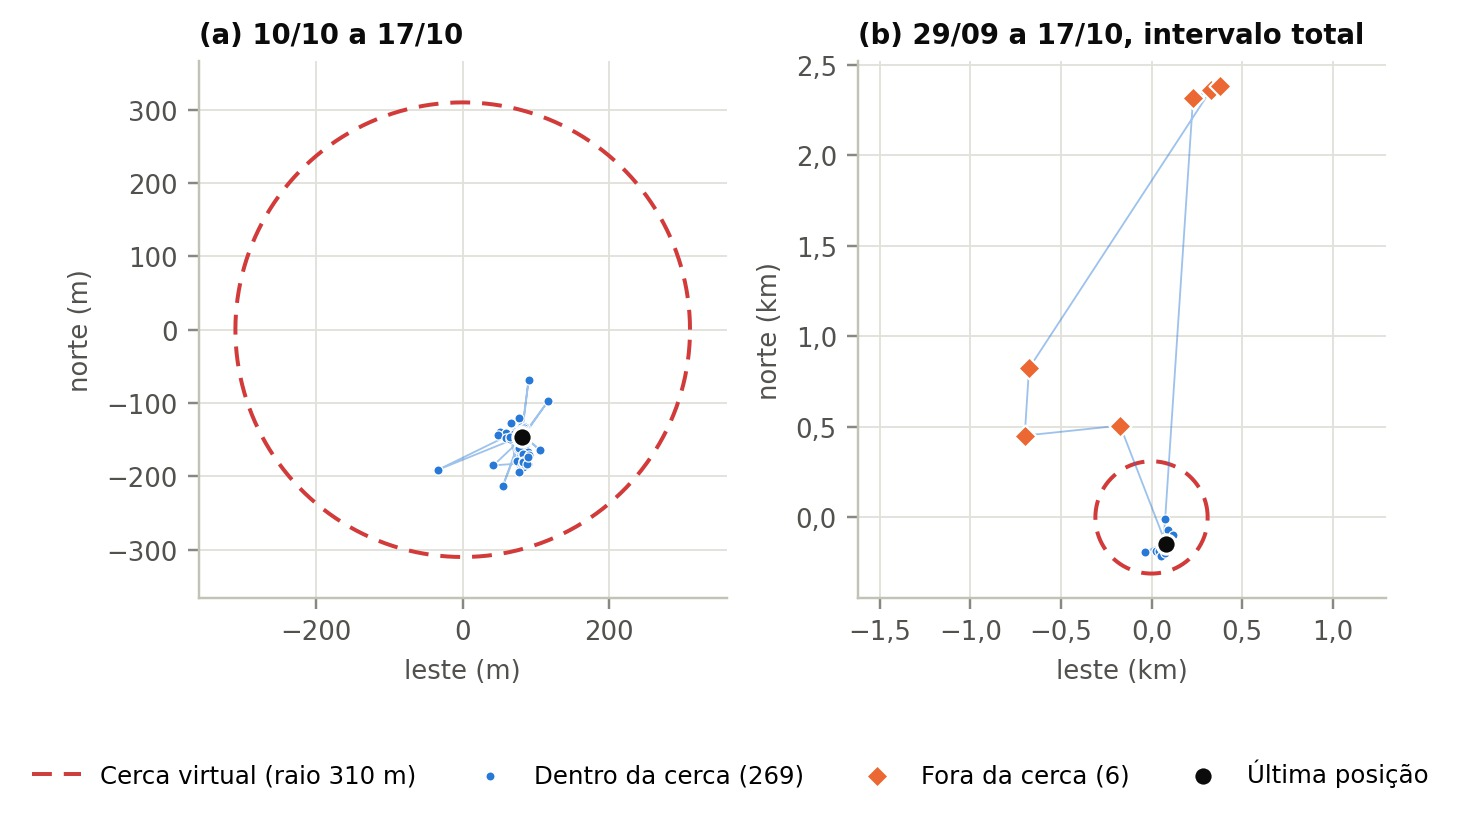
\includegraphics[width=\textwidth]{figuras/uc1_trajeto.jpg}
  \fonte{Elaborado pelo autor (2026).}
\end{figure}

Seis posições ficaram fora da cerca, todas em 30/09, entre 13h32 e 14h31, a até 2,41 km do centro. O site registrou o alerta de saída da cerca a partir da primeira delas: o cartão de localização do cavalo passou a indicar ``Fora da cerca'' e o alerta apareceu no sino do portal. Nas demais 269 posições a \textit{tag} estava dentro do raio.

A Figura~\ref{fig:uc1-dia} mostra quantas posições chegaram em cada dia. A quantidade variou de 6 a 75 por dia. A rede Find Hub depende de celulares Android que passem perto da \textit{tag}, e o servidor só registra o que a rede entrega.

\begin{figure}[htb]
  \centering
  \caption{Posições recebidas por dia, dentro e fora da cerca}
  \label{fig:uc1-dia}
  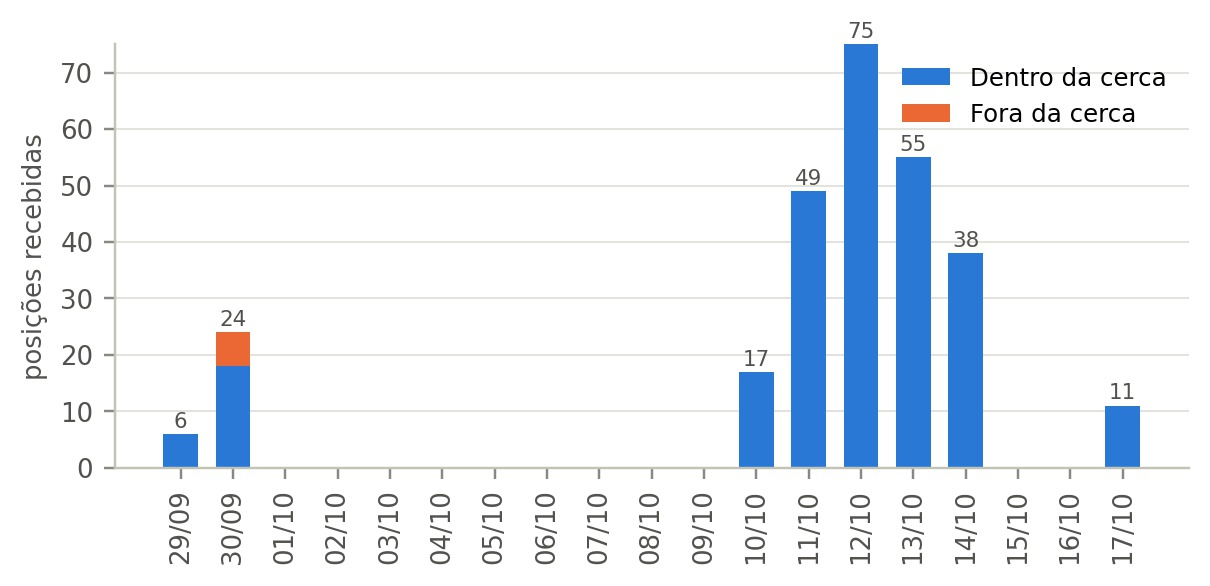
\includegraphics[width=\textwidth]{figuras/uc1_por_dia.jpg}
  \fonte{Elaborado pelo autor (2026).}
\end{figure}

A Figura~\ref{fig:uc1-intervalo} apresenta o intervalo entre posições consecutivas e a precisão informada pela rede em cada posição. O intervalo mediano foi de 16 min, e 90\% dos intervalos ficaram abaixo de 57 min; o maior intervalo, de 239 h, corresponde à lacuna entre 30/09 e 10/10. A precisão informada teve mediana de 75 m, e 46\% das posições chegaram com o valor máximo aceito pelo filtro do servidor, 100 m.

\begin{figure}[htb]
  \centering
  \caption{Intervalo entre posições consecutivas e precisão informada pela rede}
  \label{fig:uc1-intervalo}
  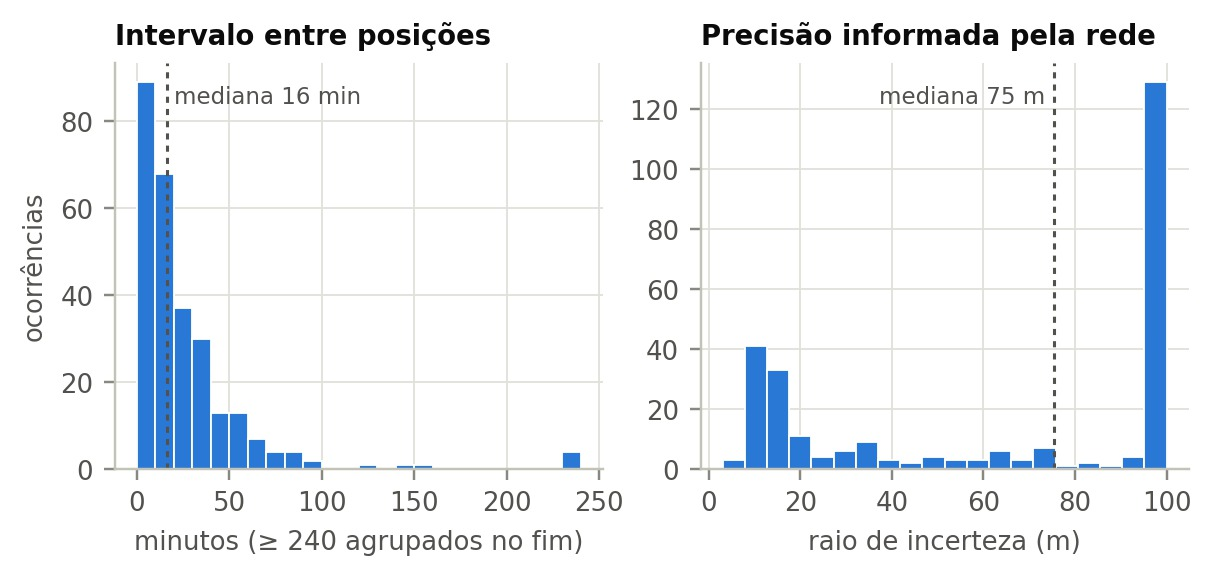
\includegraphics[width=\textwidth]{figuras/uc1_intervalo_precisao.jpg}
  \fonte{Elaborado pelo autor (2026).}
\end{figure}

\subsection{Incerteza da posição}
\label{sec:uc1-incerteza-posicao}

A incerteza foi avaliada pela análise de amostra única de \citeonline{moffat1988}: cada posição é uma leitura isolada, e a dispersão do sistema de medição é obtida de um experimento auxiliar feito em condição representativa. O experimento auxiliar foi o período de 10/10 a 17/10, com a \textit{tag} parada no mesmo ponto e 243 leituras. As coordenadas foram convertidas para metros nas direções leste ($x$) e norte ($y$), e o desvio-padrão amostral de cada direção foi $S_x = 9{,}6$~m e $S_y = 14{,}0$~m.

Com 242 graus de liberdade, a distribuição qui-quadrado limita o desvio-padrão da população a $0{,}92\,S \le \sigma \le 1{,}10\,S$, ao nível de 95\% \cite{moffat1988}. Foi adotado o valor mais provável, $\sigma = S$. A incerteza de uma leitura isolada, a 95\% de confiança (chance de 20 para 1), é
\begin{equation}
  \delta x = 2\sigma_x = 19{,}2~\text{m}, \qquad \delta y = 2\sigma_y = 27{,}9~\text{m}.
  \label{eq:uc1-incerteza-posicao}
\end{equation}
Com o limite superior de $\sigma$, os valores seriam 21,0 m e 30,6 m. Nos dados, 96,3\% das leituras ficaram dentro de $\pm\delta x$ e 92,2\% dentro de $\pm\delta y$. A distribuição não é gaussiana, pois 92\% das leituras na direção leste ficaram dentro de $\pm S_x$, e uma leitura isolada se afastou 121 m da média. A autocorrelação entre leituras consecutivas foi de $-0{,}001$ (leste) e $0{,}12$ (norte), e as leituras foram tratadas como independentes, condição exigida para a soma quadrática.

A Tabela~\ref{tab:uc1-ordens} separa a incerteza da posição nas três ordens de \citeonline{moffat1988}. A ordem zero corresponde à resolução dos valores recebidos, que chegam com $10^{-7}$ grau (cerca de 1,1 cm), e a incerteza instrumental é a metade da resolução \cite{poiate}. O horário de cada posição chega em segundos inteiros, com incerteza de 0,5 s. A primeira ordem é a dispersão medida no experimento auxiliar. Na ordem $N$ entraria o erro fixo da rede, isto é, a diferença entre a média das leituras e a posição verdadeira da \textit{tag}. Esse erro não foi medido, porque não havia uma referência de posição com incerteza menor; ele desloca todas as leituras da mesma forma, e por isso se cancela nas diferenças entre posições usadas na distância e na velocidade, mas afeta a verificação da cerca.

\begin{table}[htb]
  \centering
  \caption{Incerteza de uma posição a 95\% de confiança}
  \label{tab:uc1-ordens}
  \begin{tabular}{lrrl}
    \hline
    \textbf{Ordem} & \textbf{Leste (m)} & \textbf{Norte (m)} & \textbf{Origem} \\
    \hline
    Zero & 0,005 & 0,006 & resolução de $10^{-7}$ grau \\
    Primeira & 19,2 & 27,9 & experimento auxiliar, $2S$ \\
    $N$ & 19,2 & 27,9 & erro fixo da rede não avaliado \\
    \hline
  \end{tabular}
  \fonte{Elaborado pelo autor (2026).}
\end{table}

A ordem zero é cerca de 4 mil vezes menor que a primeira e foi desprezada, pois uma parcela menor que um terço da maior tem efeito pequeno na soma quadrática \cite{moffat1988}. Em 95,9\% das leituras paradas, a distância até a média ficou abaixo da precisão informada pela rede para aquela leitura, cuja mediana foi de 75 m. A precisão informada se comporta como um limite conservador, maior que a incerteza medida.

\subsection{Verificação da cerca com a incerteza}

A cerca virtual funciona como uma tolerância: a posição é aceita enquanto a distância $r$ até o centro não passa do raio $R = 310$~m. Seguindo \citeonline{poiate}, a incerteza de medição divide a faixa em três zonas. A zona de aceitação vai até $R - \delta r$, a zona de rejeição começa em $R + \delta r$ e, entre as duas, fica a zona de dúvida, onde a medição não permite afirmar se a \textit{tag} está dentro ou fora. A incerteza da distância ao centro vem da propagação das incertezas da Equação~\eqref{eq:uc1-incerteza-posicao}:
\begin{equation}
  \delta r = \sqrt{\left(\frac{x}{r}\,\delta x\right)^2 + \left(\frac{y}{r}\,\delta y\right)^2}.
  \label{eq:uc1-incerteza-raio}
\end{equation}

O maior valor de $\delta r$ entre as posições foi de 27,8 m, o que coloca a zona de dúvida entre 282 m e 338 m. A incerteza ficou abaixo de um décimo do intervalo de tolerância (31 m), critério de equilíbrio entre custo e qualidade recomendado por \citeonline{poiate}. A Figura~\ref{fig:uc1-zonas} mostra a distância de cada posição ao centro com as três zonas.

\begin{figure}[htb]
  \centering
  \caption{Distância das posições ao centro da cerca, com as zonas de aceitação, dúvida e rejeição}
  \label{fig:uc1-zonas}
  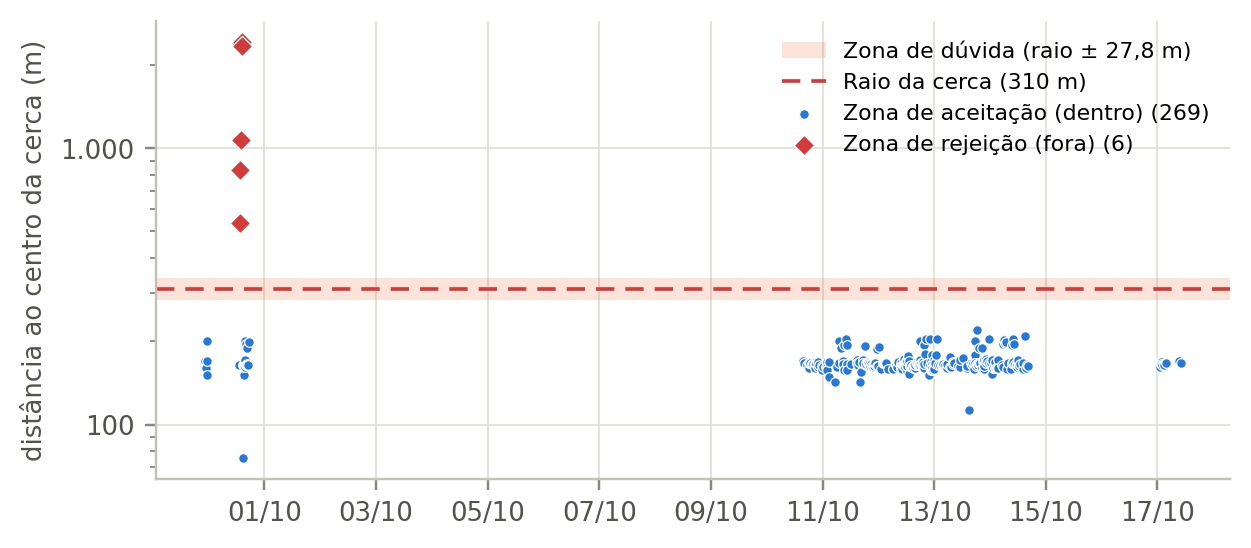
\includegraphics[width=\textwidth]{figuras/uc1_zonas.jpg}
  \fonte{Elaborado pelo autor (2026).}
\end{figure}

As 269 posições dentro da cerca ficaram a até 220 m do centro, na zona de aceitação. As seis posições de 30/09 ficaram a pelo menos 536 m, na zona de rejeição, e nenhuma posição caiu na zona de dúvida. O alerta de saída da cerca de 30/09 não depende, portanto, da incerteza da posição.

\subsection{Parâmetros calculados pelo site}

O site calcula, a partir das posições gravadas no banco, quatro parâmetros para o intervalo escolhido. A distância percorrida é a soma das distâncias entre posições consecutivas, $d = \sum_k s_k$. A velocidade média é essa distância dividida pelo tempo $T$ entre a primeira e a última posição. A velocidade máxima é a maior razão $s_k/\Delta t_k$ entre duas posições consecutivas. A aceleração média é a média das variações de velocidade entre trechos seguidos.

A incerteza desses resultados foi propagada pelo método da perturbação sequencial \cite{moffat1988}, aplicado à mesma função de cálculo do site. Cada entrada $X_i$ (latitude, longitude e horário de cada posição) foi aumentada e reduzida pela sua incerteza $\delta X_i$, uma de cada vez, e a contribuição $C_i$ foi tomada como a média de $|R_{i+} - R_0|$ e $|R_{i-} - R_0|$, porque o resultado não é linear nas posições. A incerteza do resultado é a soma quadrática das contribuições,
\begin{equation}
  \delta R = \sqrt{\sum_i C_i^2}, \qquad C_i \approx \frac{\partial R}{\partial X_i}\,\delta X_i,
  \label{eq:uc1-perturbacao}
\end{equation}
e tem o mesmo nível de confiança das entradas, 95\%. Para a velocidade média, a propagação analítica da apostila de \citeonline{poiate},
\begin{equation}
  \frac{\delta \bar v}{\bar v} = \sqrt{\left(\frac{\delta d}{d}\right)^2 + \left(\frac{\delta T}{T}\right)^2},
  \label{eq:uc1-vmed}
\end{equation}
com $\delta T = 1$~s (metade da resolução em cada extremo), deu o mesmo valor que a perturbação sequencial até a terceira casa. A parcela do horário foi desprezível em todos os resultados, exceto na velocidade máxima de 13/10, em que foi de 23 km/h contra 128 km/h da parcela das posições.

A soma de passos tem também um erro fixo, que \citeonline{moffat1988} classifica como erro conceitual: com a \textit{tag} parada, o ruído da posição gera passos de comprimento não nulo, e o site os soma como distância. Esse erro foi medido no experimento auxiliar, com 121 pares de leituras consecutivas sem leitura em comum. O passo médio foi de $(14{,}0 \pm 3{,}3)$~m, em que a incerteza é $t\,S/\sqrt{N}$, com $t = 1{,}98$ para 120 graus de liberdade. Para um intervalo com $k$ passos, o erro fixo é $B = k \times 14{,}0$~m, e a sua incerteza, $k \times 3{,}3$~m, somada de forma linear, porque o mesmo valor médio é usado em todos os passos. A distância corrigida é $d - B$, e a sua incerteza de ordem $N$ é a soma quadrática da incerteza propagada com a incerteza de $B$. Essa correção supõe a \textit{tag} parada em todos os passos e, nos dias com deslocamento, superestima o erro fixo. A velocidade média recebe a mesma correção, dividida por $T$.

A Figura~\ref{fig:uc1-parametros} apresenta, por dia, o valor calculado pelo site, a incerteza expandida e o erro fixo. Um valor foi considerado significativo quando superou a sua incerteza, isto é, quando a diferença em relação a zero (ou ao erro fixo, no caso da distância e da velocidade média) foi maior que a incerteza dessa diferença \cite{moffat1988}.

\begin{figure}[htb]
  \centering
  \caption{Parâmetros calculados pelo site por dia, com a incerteza expandida e o erro fixo}
  \label{fig:uc1-parametros}
  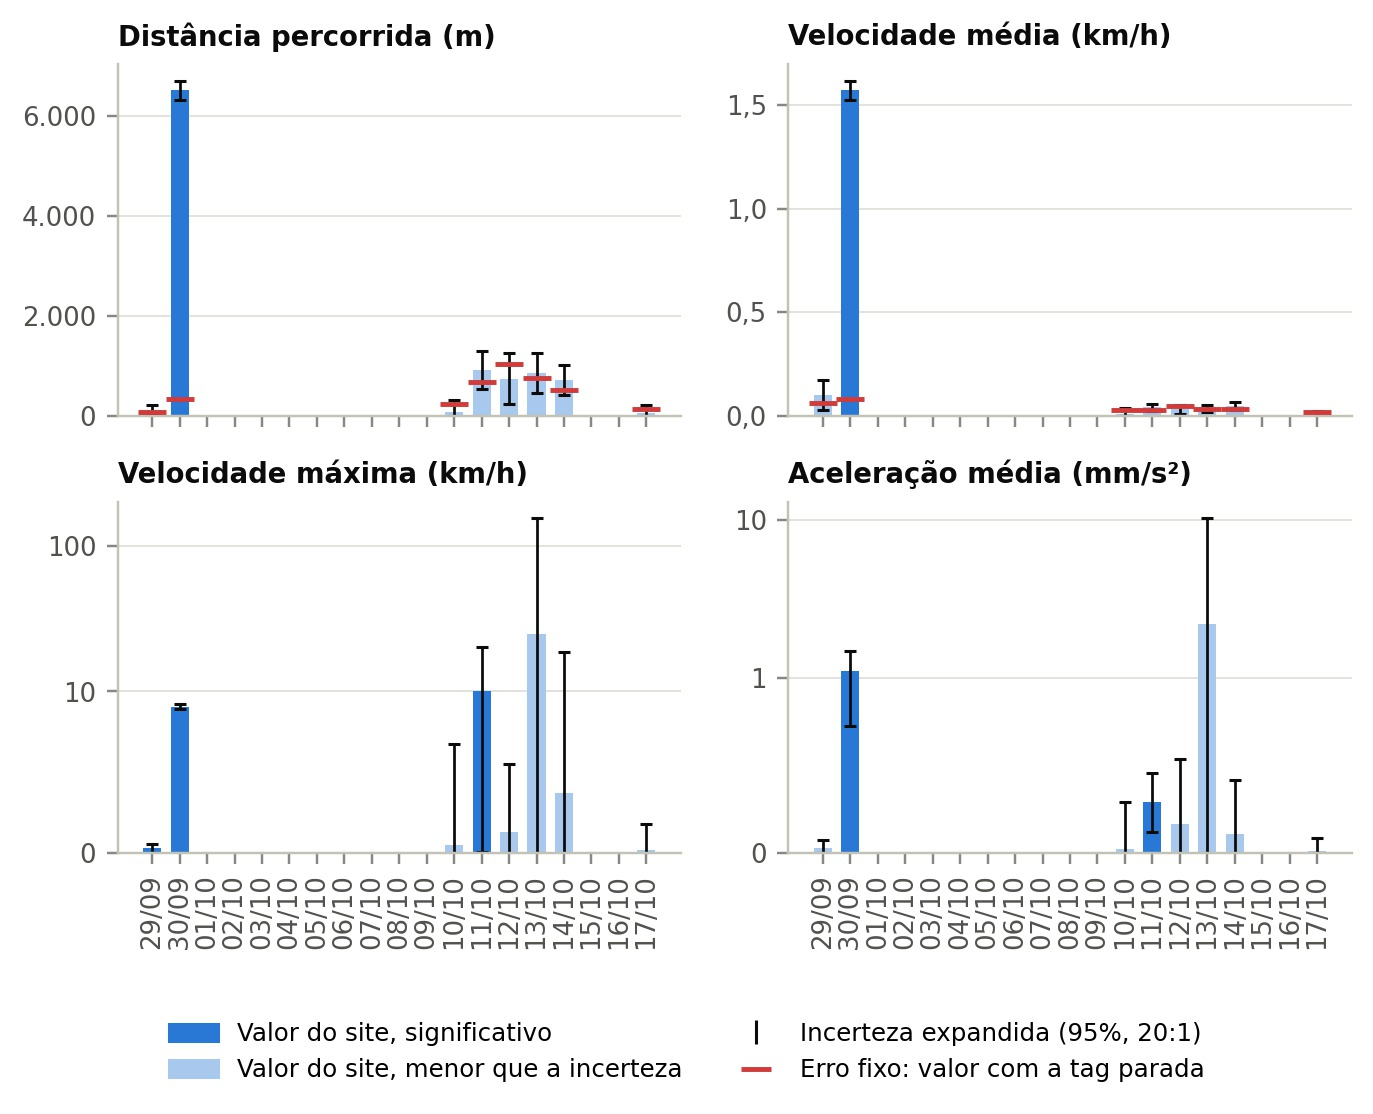
\includegraphics[width=\textwidth]{figuras/uc1_parametros.jpg}
  \fonte{Elaborado pelo autor (2026).}
\end{figure}

A Tabela~\ref{tab:uc1-dia30} reúne os resultados de 30/09, o dia com deslocamento, em 24 posições e 4 h 08 min. Todos os parâmetros foram significativos. A distância corrigida foi de $(6{,}19 \pm 0{,}19)$~km, com incerteza relativa de 3\%.

\begin{table}[htb]
  \centering
  \caption{Parâmetros de 30/09 a 95\% de confiança}
  \label{tab:uc1-dia30}
  \begin{tabular}{lrrr}
    \hline
    \textbf{Parâmetro} & \textbf{Valor do site} & \textbf{Erro fixo} & \textbf{Valor corrigido} \\
    \hline
    Distância percorrida & $(6{,}51 \pm 0{,}17)$ km & $(0{,}32 \pm 0{,}08)$ km & $(6{,}19 \pm 0{,}19)$ km \\
    Velocidade média & $(1{,}57 \pm 0{,}04)$ km/h & 0,08 km/h & $(1{,}50 \pm 0{,}05)$ km/h \\
    Velocidade máxima & $(9{,}0 \pm 0{,}2)$ km/h & --- & --- \\
    Aceleração média & $(1{,}1 \pm 0{,}4)$ mm/s² & --- & --- \\
    \hline
  \end{tabular}
  \fonte{Elaborado pelo autor (2026).}
\end{table}

Nos dias com a \textit{tag} parada, a distância corrigida foi compatível com zero. Em 11/10, por exemplo, o site somou 914 m, o erro fixo foi de 674 m e a distância corrigida, $(240 \pm 370)$~m. A velocidade máxima de 11/10, $(10 \pm 10)$~km/h, ficou no limite da significância, e a de 13/10, 24,7 km/h, teve incerteza de 130 km/h, porque vem de duas posições recebidas com poucos segundos de diferença. A Tabela~\ref{tab:uc1-total} reúne os parâmetros do intervalo total.

\begin{table}[htb]
  \centering
  \caption{Parâmetros calculados pelo site no intervalo total (29/09 a 17/10), a 95\% de confiança}
  \label{tab:uc1-total}
  \begin{tabular}{lrrr}
    \hline
    \textbf{Parâmetro} & \textbf{Valor do site} & \textbf{Erro fixo} & \textbf{Valor corrigido} \\
    \hline
    Distância percorrida & $(10{,}1 \pm 0{,}8)$ km & $(3{,}8 \pm 0{,}9)$ km & $(6{,}2 \pm 1{,}2)$ km \\
    Velocidade média & $(0{,}024 \pm 0{,}002)$ km/h & 0,009 km/h & $(0{,}015 \pm 0{,}003)$ km/h \\
    Velocidade máxima & $(25 \pm 130)$ km/h & --- & --- \\
    Aceleração média & $(0{,}7 \pm 1{,}7)$ mm/s² & --- & --- \\
    \hline
  \end{tabular}
  \fonte{Elaborado pelo autor (2026).}
\end{table}

A distância corrigida do intervalo total, $(6{,}2 \pm 1{,}2)$~km, coincide com a de 30/09: o restante dos 10,1 km somados pelo site corresponde ao ruído da posição nos dias parados. Um passo de comprimento próximo de zero tem incerteza de $\sqrt{2}\,\delta y = 39{,}5$~m, e 243 dos 274 passos do intervalo ficaram abaixo desse valor. A velocidade máxima e a aceleração média do intervalo total têm incerteza maior que o próprio valor e não permitem conclusões.

Com intervalos medianos de 16 min e incerteza de 19 m (leste) e 28 m (norte) a 95\% de confiança, a localização pela rede Find Hub atende à verificação da cerca virtual, sem posições na zona de dúvida. Para medir distância e velocidade em treinos, o cálculo do site precisaria descontar o erro fixo ou descartar passos menores que a incerteza de um passo, ou essas grandezas teriam de vir do acelerômetro.
